\chapter[\cedczeroshorttitle{}]{\cedczerolongtitle{}}

\label{cedc0}

\beginchapterquote{``True genius resides in the capacity for evaluation of uncertain,
                     hazardous, and conflicting information.''}
                     {Winston Churchill}
					 \index{Churchill, Winston}

%%%%%%%%%%%%%%%%%%%%%%%%%%%%%%%%%%%%%%%%%%%%%%%%%%%%%%%%%%%%%%%%%%%%%%%%%%%%%%%%
%%%%%%%%%%%%%%%%%%%%%%%%%%%%%%%%%%%%%%%%%%%%%%%%%%%%%%%%%%%%%%%%%%%%%%%%%%%%%%%%
%%%%%%%%%%%%%%%%%%%%%%%%%%%%%%%%%%%%%%%%%%%%%%%%%%%%%%%%%%%%%%%%%%%%%%%%%%%%%%%%
\section{Introduction}
%Section tag: INT0
\label{cedc0:sint0}

In microcontroller work, it is frequently necessary to consider how
best to add redundancy to data.  The following design scenarios are
common.

\begin{enumerate}
\item Immediately on powerup, a microcontroller product calculates
      the checksum of its program memory (usually ROM or FLASH) and compares this
      checksum to a stored value in order to detect possible corruption of program
      memory.  What is the best way to calculate a checksum for this
      purpose?
\item A storage medium that will tolerate a limited number of write cycles
      (such as EEPROM), will used to used to store data which will change 
      and need to rewritten more times than the life of the medium will
      accomodate.  As a result, a strategy which wears out a portion of the medium
      and then uses another portion is employed.  When a portion of the medium
      wears out (as evidenced by corruption of bits), how can the data be 
      reliably recovered before
      being transferred to the next portion?
\item A microcontroller product stores data in battery-backed RAM while powered
      down.   What type of checksum should be added to this data to provide the maximum
      protection against data corruption?
\item Microcontrollers on the same circuit board communicate with each other
      using UARTs.  What form of checksum should be used to add protection
      against electrical noise?
\end{enumerate}


This chapter deals with the mathematical basis for four
questions.

\begin{enumerate}
\item What is the mathematical basis for redundancy to allow error
      detection and error correction?
\item How can redundancy be added to data to enable detection of errors?
\item How can redundancy be added to data to enable correction of
      errors?
\item How can adding redundancy (encoding) and detecting and correcting
      errors (decoding) be performed efficiently in 
      microcontroller software?
\end{enumerate}

Note that although the results presented in this chapter for the most part
have their origins in the study of communication channels, the problem of 
protecting computer storage that may degrade (disc, tape, battery-backed RAM,
EEPROM, etc.) is mathematically the same problem as protecting data transmitted
through a communication channel.  In either case $k$ data bits are protected
by $n-k$ check bits (see Figure \ref{fig:cedc0:scon0:sccb0:01}), 
and the essence of the mathematical problem is how best to
select the check bits.


%%%%%%%%%%%%%%%%%%%%%%%%%%%%%%%%%%%%%%%%%%%%%%%%%%%%%%%%%%%%%%%%%%%%%%%%%%%%%%%%
%%%%%%%%%%%%%%%%%%%%%%%%%%%%%%%%%%%%%%%%%%%%%%%%%%%%%%%%%%%%%%%%%%%%%%%%%%%%%%%%
%%%%%%%%%%%%%%%%%%%%%%%%%%%%%%%%%%%%%%%%%%%%%%%%%%%%%%%%%%%%%%%%%%%%%%%%%%%%%%%%
\section{Coding Concepts}
%Section tag: con0
\label{cedc0:scon0}

\index{coding theory}\emph{Coding theory} is the branch of mathematics 
concerned with transmitting data across noisy channels and recovering
the data \cite{bibref:w:ctfirst50}.  In this section we introduce the
basic concepts and terminology which apply to microcontroller work.


%%%%%%%%%%%%%%%%%%%%%%%%%%%%%%%%%%%%%%%%%%%%%%%%%%%%%%%%%%%%%%%%%%%%%%%%%%%%%%%%
%%%%%%%%%%%%%%%%%%%%%%%%%%%%%%%%%%%%%%%%%%%%%%%%%%%%%%%%%%%%%%%%%%%%%%%%%%%%%%%%
%%%%%%%%%%%%%%%%%%%%%%%%%%%%%%%%%%%%%%%%%%%%%%%%%%%%%%%%%%%%%%%%%%%%%%%%%%%%%%%%
\subsection{Bits, Communication Channels, Messages, And Check Bits}
%Subection tag: ccb0
\label{cedc0:scon0:sccb0}

We assume that the data we wish to transmit is an ordered sequence of \index{bit}bits.
Each bit is a symbol of the \index{binary alphabet}binary alphabet, 
$\mathbb{B} = \{0,1\}$.  Many results in coding theory have been generalized to
alphabets with more than two symbols, but for microcontroller work it is adequate
to consider only $\mathbb{B}$, and in this chapter only
$\mathbb{B}$ is considered.

Bits are transmitted through a \index{communication channel}\index{channel}%
\emph{communication channel} (or simply \emph{channel}), which may with probability $p$
corrupt a transmitted bit from 0 to 1 or vice-versa; or with
probability $q=1-p$ fail to corrupt a bit.  For analysis,
we make the simplest mathematical assumptions and assume that 
the probability of corruption from 0 to 1 is the same as the probability
of corruption from 1 to 0 (i.e. $p_{0\rightarrow{}1} = p_{1\rightarrow{}0} = p$),
and that corruption of each bit is independent.  Alternately, we may imagine that rather
than being potentially corrupted during transmission, each bit is potentially 
corrupted by the degradation of computer storage.

We assume that data is transmitted in blocks of 
$n$ bits, consisting of $k$ data bits with $n-k$ check bits
(redundancy bits) appended (Figure \ref{fig:cedc0:scon0:sccb0:01}).  This concatenation of
$k$ data bits and $n-k$ check bits is called a \index{message}\emph{message}.
Most commonly
in practice, $8 \vworkdivides n,k$ (and consequently
$8 \vworkdivides (n-k)$), although this is not required.
If data is stored rather than transmitted, we may assume that
the check bits are stored at the last addresses of ROM or EEPROM.
As explained in Section \ref{cedc0:scon0:scco0},
in this chapter only codes where the checkbits are appended to the unmodified
data bits are considered.

Notationally, we treat the $n$-bit message as an ordered collection of
bits, represented by a row vector

\begin{equation}
\label{eq:cedc0:scon0:sccb0:01}
[m_0, m_1, \ldots{}, m_{n-1}] .
\end{equation}

\noindent{}(Figure \ref{fig:cedc0:scon0:sccb0:01},
includes bit notational conventions.)  $m_0$ through $m_{k-1}$ are data bits, and
$m_k$ through $m_{n-1}$ are check bits.  We may also 
treat the vector in (\ref{eq:cedc0:scon0:sccb0:01}) as 
the concatenation of data bits $d_0$ through $d_{k-1}$ and
check bits $c_0$ through $c_{n-k-1}$, in which case we use 
either of the following notations:

\begin{eqnarray}
\label{eq:cedc0:scon0:sccb0:02}
& [d_0, d_1, \ldots{}, d_{k-1}, c_0, c_1, \ldots{}, c_{n-k-1}] , & \\
\label{eq:cedc0:scon0:sccb0:02b}
& [d_0, d_1, \ldots{}, d_{k-1}] | [c_0, c_1, \ldots{}, c_{n-k-1}] . &
\end{eqnarray}

Implicit in
this model is the assumption that a framing error (where communication hardware or 
software misidentifies a block of data in time) is much less probable than
a collection of bit errors which overwhelm the detection/correction 
capability of the $n-k$ check bits.  There are in fact some 
scenarios\footnote{One classic example is the CAN bit-stuffing vulnerability which can
with some data patterns lower the Hamming distance of CAN to 2.}
where mechanisms exist to circumvent the function of the check bits by creating 
framing errors.
By their nature, such scenarios involve the corruption of a small number of bits 
(or samples) in a way so as to generate a framing error and shift a large number of bits
right or left.  We assume for analytic convenience that the probability of 
a framing error is much less than the probability of the corruption of enough bits 
to overwhelm the capability of the check bits.  However, experience has shown that 
this assumption needs to be verified, as many practical communication protocols have
framing weaknesses.\footnote{Note that the notion of a framing error does not apply 
to a medium that does not use start and end markers that might be misinterpreted.
For example, ROM or EEPROM have no notion of a framing error.}

\begin{figure}
\centering
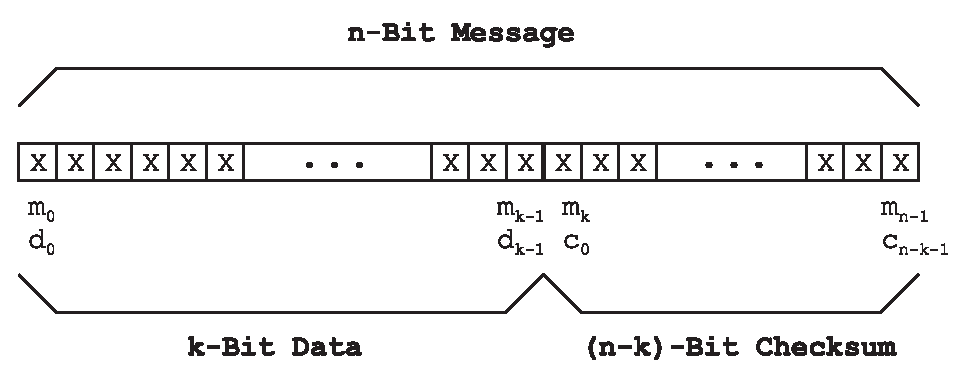
\includegraphics[width=4.6in]{c_edc0/cword01.eps}
\caption{Message Consisting Of The Concatenation Of $k$ Data Bits And $n-k$
         Check Bits, With Bit Notational Conventions}
\label{fig:cedc0:scon0:sccb0:01}
\end{figure}

We have referred to \emph{check bits} without describing the ways in which they
might be calculated.  We use the term \index{checksum}\emph{checksum} to refer
to the contiguous group of $n-k$ check bits; whether or not the bits are calculated
through summation.  In general, we impose only the requirement that the $n-k$-bit 
checksum is a deterministic function of the $k$ data bits.

We often refer to a message or a portion of a message as a 
\index{vector}\emph{vector}.  This nomenclature is appropriate because it is
convenient to treat a message as a row vector of bits.  
An 80-bit message might
be viewed as a $1 \times 80$ matrix (i.e. a row vector) with each matrix element
$\in \mathbb{B}$.  We use \emph{message} and \emph{vector} somewhat interchangeably.

We define the \index{weight}\emph{weight} of a message or vector as the number of 
1's in the message or vector.  We denote the weight of a vector or message $v$ as
$wt(v)$.


%%%%%%%%%%%%%%%%%%%%%%%%%%%%%%%%%%%%%%%%%%%%%%%%%%%%%%%%%%%%%%%%%%%%%%%%%%%%%%%%
%%%%%%%%%%%%%%%%%%%%%%%%%%%%%%%%%%%%%%%%%%%%%%%%%%%%%%%%%%%%%%%%%%%%%%%%%%%%%%%%
%%%%%%%%%%%%%%%%%%%%%%%%%%%%%%%%%%%%%%%%%%%%%%%%%%%%%%%%%%%%%%%%%%%%%%%%%%%%%%%%
\subsection[Codewords, Codes, And \protect\mbox{\protect$(n,k)$} Block Codes]
           {Codewords, Codes And \protect\mbox{\protect\boldmath$(n,k)$} Block Codes}
%Subection tag: cco0
\label{cedc0:scon0:scco0}

A \index{codeword}\emph{codeword} (as we define it here) is a message in which 
the $n-k$ check bits are consistent with the $k$ data bits.
Under this definition, all codewords are messages, but not all possible messages
are codewords.

A common cognitive misconception is that it matters in transmission or
storage whether the $k$ data bits or the $n-k$ check bits are corrupted.
It matters not.  We seek mathematical properties that apply to the messages 
and codewords, not to the $k$ data bits or $n-k$ check bits separately.

In the most general terms, a \index{code}\emph{code} is \emph{any} system
of information representation for transmission, not necessarily requiring 
transmission in fixed-length blocks.  However, in this discussion, by
\emph{code} we mean the set of all bit 
patterns with data and check bits consistent (i.e. all codewords)
which can be transmitted over a communication channel or stored
in computer memory.  For example,
$\{000, 011, 101, 110\}$ is a code.

A code may be specified either by enumeration or by rule.  For example,
we might also specify the code of the previous paragraph as 
$\{ABC: C=A \oplus B\}$.  With larger codes, enumeration is naturally not practical and
also not necessary to study the properties of interest.

An
\index{(n,k) block code@$(n,k)$ block code}\index{n,k block code@$(n,k)$ block code}%
$(n,k)$ \emph{block code} is a code where $n$ bits are transmitted (or stored) at a
time, and characterized by a function which maps from $k$ data bits to $n$ bits which
are transmitted (or stored).

In a general $(n,k)$ block code, the $n$ transmitted
bits are not required to contain or resemble the $k$ data bits; and if the $k$ data bits
are contained they are not required to have a specific order or placement within 
the $n$ transmitted bits.  Because we are interested in adding 
redundancy to ROM and in other applications
where the stored data must be contiguous and unmodified, we confine ourselves
to $(n,k)$ block codes as depicted in Figure
\ref{fig:cedc0:scon0:sccb0:01}, where the $k$ data bits are contiguous, unchanged,
in their original order, and prepended to the $n-k$ check bits.


%%%%%%%%%%%%%%%%%%%%%%%%%%%%%%%%%%%%%%%%%%%%%%%%%%%%%%%%%%%%%%%%%%%%%%%%%%%%%%%%
%%%%%%%%%%%%%%%%%%%%%%%%%%%%%%%%%%%%%%%%%%%%%%%%%%%%%%%%%%%%%%%%%%%%%%%%%%%%%%%%
%%%%%%%%%%%%%%%%%%%%%%%%%%%%%%%%%%%%%%%%%%%%%%%%%%%%%%%%%%%%%%%%%%%%%%%%%%%%%%%%
\subsection{Hamming Distance, Minimum Hamming Distance, And Errors}
%Subection tag: mhd0
\label{cedc0:scon0:smhd0}

We define the \index{Hamming distance}\emph{Hamming distance} between 
two same-length blocks $c$ and $d$, denoted $d(c,d)$, as the number of bit positions
in which the blocks differ.  Note that $d(c,d)$ is necessarily the same as the number
of 1's in $c \oplus d$.  Note also that $d(c,d)$ is the weight of the 
exclusive-OR of $c$ and $d$, i.e. $d(c,d) = wt(c \oplus d)$.  (We discuss the properties 
of the exclusive-OR function later in Section \ref{cedc0:sfft0:dff0}.)

We define the \index{minimum Hamming distance}\emph{minimum Hamming distance}
of a code, denoted $\hat{d}$, as the smallest Hamming distance between any two 
members of the code.  For example, the minimum Hamming distance of
$\{000, 011, 101, 110\}$,
denoted $\hat{d}(\{000, 011, 101, 110\})$,
 is 2, and the minimum Hamming distance of
$\{0001, 0110, 1010, 1101\}$,
denoted $\hat{d}(\{0001, 0110, 1010, 1101\})$,
 is also 2.\footnote{See Exercise 
\ref{exe:cedc0:sexe0:01}.}

We define an \index{error}\emph{error} (or alternatively, a 
\emph{bit corruption} or simply a \emph{corruption}) as the corruption
of a transmitted or stored
bit from 0 to 1 or from 1 to 0.  As mentioned in
Section \ref{cedc0:scon0:sccb0}, we assume that a corruption may occur
with probability $p$ or fail to occur with probability $q=1-p$.

We define a \index{message corruption}\emph{message corruption} or simply 
\emph{corruption} as the corruption of one or more bits within the message
during transmission or storage.
Note that the minimum Hamming distance $\hat{d}$ of a code
guarantees that at least $\hat{d}$ errors are required to transform
one codeword into another, thus guaranteeing that any corruption
of $\hat{d}-1$ or fewer bits is detectable.

If the errors within a message are distributed in a special way, we may be
able to devise codes that are more resistant to these special distributions 
than to an arbitrary distribution of errors.  One such special distribution
is a \index{burst error}\emph{burst error}.  A \emph{burst error of length $b$}
is defined as any number of errors in a span of $b$ bits.  For example, corruption of
00001111 to 00011001 represents a burst error of length 4 (the corruptions are in 
the 4th, 6th, and 7th bits, which span 4 bits inclusive).  A burst error may naturally
span no fewer than 1 bit and no more than $n$ bits.

We are very careful \emph{not} to define a codeword as an
uncorrupted message.  No code except a code consisting of only one codeword
can sustain an unlimited number of bit corruptions while still guaranteeing
that the message corruption will be detectable.\footnote{This observation that
a single-codeword code can sustain an unlimited number of bit corruptions is a
mathematical fallacy and a semantic parlor trick.  An $(n,k)$ block code with only
one code word effectively has a maximum Hamming distance $\hat{d}$ of $n$ plus the number
of framing bits, stop bits, etc. in the message as transmitted.  Sufficient noise
in a communication channel may cause communication hardware to believe the
codeword was transmitted when in fact it was not.  See the remarks regarding
framing weaknesses in Section \ref{cedc0:scon0:sccb0}.}  A codeword may in fact
be a corrupted message where the number of bit corruptions has overwhelmed the 
minimum Hamming distance $\hat{d}$ of the code so as to transform one codeword
into another.

Generally, error-detecting and error-correcting codes
(Section \ref{cedc0:scon0:secv0}) must be selected with some knowledge 
of the error
rates of the 
communication channel or storage medium.  Noisier communication channels 
or poorer storage mediums require codes with
better error-detecting and/or error-correcting properties.  Normally, the design goal
is to achieve a very low probability of undetected corruption or uncorrectable corruption.


%%%%%%%%%%%%%%%%%%%%%%%%%%%%%%%%%%%%%%%%%%%%%%%%%%%%%%%%%%%%%%%%%%%%%%%%%%%%%%%%
%%%%%%%%%%%%%%%%%%%%%%%%%%%%%%%%%%%%%%%%%%%%%%%%%%%%%%%%%%%%%%%%%%%%%%%%%%%%%%%%
%%%%%%%%%%%%%%%%%%%%%%%%%%%%%%%%%%%%%%%%%%%%%%%%%%%%%%%%%%%%%%%%%%%%%%%%%%%%%%%%
\subsection{Error-Detecting Versus Error-Correcting Codes}
%Subection tag: ecv0
\label{cedc0:scon0:secv0}

An \index{error-detecting code}\emph{error-detecting code} is a code which is
designed so that message errors
(a message which is not a codeword) will be detected but not corrected.  
Error-detecting codes are attractive
when there is the opportunity to request that the transmitter retransmit the 
corrupted data, or when obtaining a correct copy of the data is not important but
detecting (and perhaps discarding) corrupted data is important.

An \index{error-correcting code}\emph{error-correcting code} is a code designed 
so that message errors can be both detected and corrected.  Error-correcting 
codes are attractive when 
there is no opportunity for retransmission of the corrupted data, but possessing
a correct copy of the data is important.  Example attractive 
applications of error-correcting codes are compact disc audio data (where the
CD should play even with scratches, and there is no opportunity to obtain
retransmission of the data) and data transmitted from space exploration satellites
(where the signal-to-noise ratio is low, and there is not opportunity for retransmission
or perhaps not even two-way communication).

In this section we show the required relationship between minimum Hamming
distance $\hat{d}$ and the error-detecting and error-correcting capabilities
of a code.

We define the \index{error-detecting capability of a code}\index{code!error-detecting capability}%
\emph{error-detecting capability} $d_{ED}$ of a code as the largest number of bit errors 
in a message which will \emph{always} be detectable.  It follows
immediately and intuitively that 

\begin{equation}
\label{eq:cedc0:scon0:secv0:01}
d_{ED} = \hat{d} - 1 .
\end{equation}

\noindent{}If the minimum 
Hamming distance of a code is $\hat{d}$, then there exists at least
one pair of codewords
$c_1, c_2$ such that $d(c_1, c_2) = \hat{d}$.  Thus it is possible to corrupt
$c_1$ into $c_2$ with $\hat{d}$ corrupted bits and therefore
$d_{ED} < \hat{d}$.  On the other hand, the minimum Hamming distance 
$\hat{d}$ guarantees that it is \emph{not} possible to corrupt from one codeword to another
with only $\hat{d}-1$ bit corruptions.  Therefore
(\ref{eq:cedc0:scon0:secv0:01}) is true.

We define the \index{error correcting capability of a code}\index{code!error correcting capability}%
\emph{error correcting capability} $d_{EC}$ of a code  as the largest number of bit errors 
in a message which will \emph{always} be correctable.  By \emph{correctable} we mean
that we can recover the original $n$-bit codeword into which errors were introduced.

To illustrate the relationship between Hamming distance and the error correcting
capability of a code, consider the code $\{000, 111\}$ depicted in
Figure \ref{fig:cedc0:scon0:secv0:01}.  In the figure, each edge in the cube depicts
a single bit error which may occur in a message.  Each vertex in the cube 
represents a message.

\begin{figure}
\centering
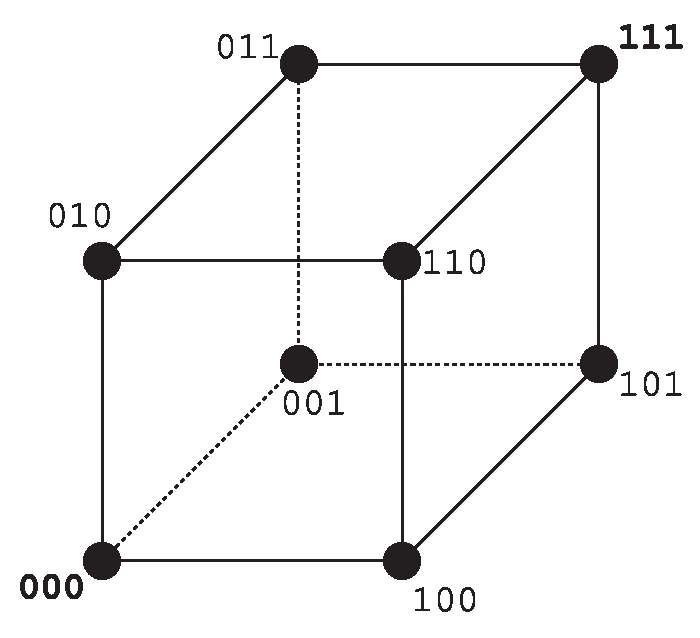
\includegraphics[height=2.5in]{c_edc0/cube01.eps}
\caption{Three-Dimensional Cube Illustrating Error Correction With Code $\{000, 111\}$}
\label{fig:cedc0:scon0:secv0:01}
\end{figure}

Note that the minimum Hamming $\hat{d}$ distance of the code $\{000, 111\}$ is 3:  in
Figure \ref{fig:cedc0:scon0:secv0:01} one must travel along three edges
(corresponding to three bit errors) in order to travel from 000 to 111 or back.

If we claim that a code has an error correcting capability of $d_{EC}$, 
then any corruption of a codeword by $d_{EC}$ errors must be correctable.
To be \emph{correctable} means that if we guess based on the corrupted
codeword what the original codeword is, we must always be able to guess
correctly.  This notion implies that the original codeword must be the 
closest codeword (as measured by number of bit corruptions) to the corrupted codeword.

This notion of \emph{closest} codeword leads to the notion of a \emph{packing sphere}.
A \emph{packing sphere of radius $\rho$} is the set of all messages
at a distance of $\rho$ or less from a given codeword.  In order for 
a code to have an error correcting capability of $d_{EC}=\rho$, 
the packing spheres or radius $\rho$ about all codewords must be disjoint.
This ensures that any message at a distance $d_{EC}$ or less from a codeword
does, in fact, have a \emph{nearest} codeword.

Figure \ref{fig:cedc0:scon0:secv0:02} is
Figure \ref{fig:cedc0:scon0:secv0:01} redrawn to show the packing spheres of
radius $\rho=1$ about the two codewords 000 and 111.  The code
$\{000,111\}$ depicted in Figures \ref{fig:cedc0:scon0:secv0:01} and
\ref{fig:cedc0:scon0:secv0:02} has an error correcting capability of 
$d_{EC}=1$.  For error correction, any message in the packing sphere
about 000 must be mapped back to 000, and any message in the packing sphere
about 111 must be transformed back to 111.

\begin{figure}
\centering
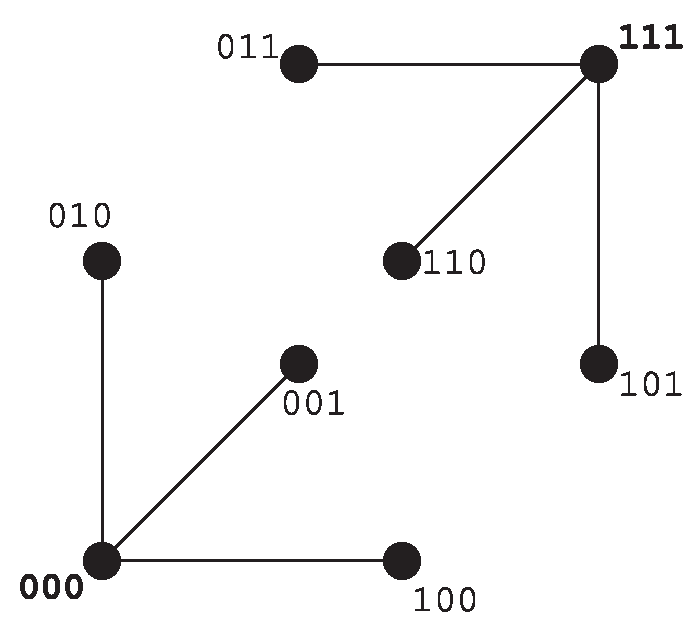
\includegraphics[height=2.5in]{c_edc0/cube02.eps}
\caption{Packing Spheres Of Radius $\rho{}=1$ About Codewords 000 And 111}
\label{fig:cedc0:scon0:secv0:02}
\end{figure}

The requirement for disjointness of packing spheres immediately leads to
the constraint

\begin{equation}
\label{eq:cedc0:scon0:secv0:02}
\hat{d} > 2 \rho 
\end{equation}

\noindent{}or equivalently when considering only integers that

\begin{equation}
\label{eq:cedc0:scon0:secv0:03}
\hat{d} \geq 2 \rho + 1 . 
\end{equation}

\noindent{}Since the radius $\rho$ of the packing sphere is 
equivalent to the error correcting capability $d_{EC}$ of
a code, we may equivalently write 
(\ref{eq:cedc0:scon0:secv0:02}) and (\ref{eq:cedc0:scon0:secv0:03})
as $\hat{d} > 2 d_{EC}$ and $\hat{d} \geq 2 d_{EC} + 1$, respectively.

(\ref{eq:cedc0:scon0:secv0:02}) and (\ref{eq:cedc0:scon0:secv0:03})
treat minimum Hamming distance $\hat{d}$ as a function of 
the packing sphere radius $\rho$.  With a known minimum Hamming distance 
$\hat{d}$, one may also calculate the largest disjoint
packing spheres that can be constructed:

\begin{equation}
\label{eq:cedc0:scon0:secv0:04}
d_{EC} = \rho = \left\lfloor {\frac{\hat{d}-1}{2}} \right\rfloor .
\end{equation}

This section has demonstrated the relationship between the minimum Hamming
distance $\hat{d}$ of a code and the error detection capability of the code
(Equation \ref{eq:cedc0:scon0:secv0:01}), as well as the relationship between the
minimum Hamming
distance $\hat{d}$ and the error correction capabilility 
(Equations \ref{eq:cedc0:scon0:secv0:02} through 
\ref{eq:cedc0:scon0:secv0:04}).

Note that the relationships derived do apply to the example presented in 
Figures \ref{fig:cedc0:scon0:secv0:01} and \ref{fig:cedc0:scon0:secv0:02}.
The code shown in the figures has a minimum Hamming distance $\hat{d}=3$.
(\ref{eq:cedc0:scon0:secv0:01}) predicts that this code should have
an error detection capability of $d_{ED}=2$, which is the case.  
(\ref{eq:cedc0:scon0:secv0:04}) predicts that this code should have an error correction
capability $d_{EC}=1$, which is also the case and can be verified by
examining Figure \ref{fig:cedc0:scon0:secv0:02}.

In the code presented in Figures \ref{fig:cedc0:scon0:secv0:01} and 
\ref{fig:cedc0:scon0:secv0:02}, the union of all packing spheres of radius 
$\rho=1$ contains all messages (i.e. there are no messages which are not part of
a packing sphere).  Such a code is called a \emph{perfect code}.  Most codes
are not perfect codes, and this will be discussed later.


%%%%%%%%%%%%%%%%%%%%%%%%%%%%%%%%%%%%%%%%%%%%%%%%%%%%%%%%%%%%%%%%%%%%%%%%%%%%%%%%
%%%%%%%%%%%%%%%%%%%%%%%%%%%%%%%%%%%%%%%%%%%%%%%%%%%%%%%%%%%%%%%%%%%%%%%%%%%%%%%%
%%%%%%%%%%%%%%%%%%%%%%%%%%%%%%%%%%%%%%%%%%%%%%%%%%%%%%%%%%%%%%%%%%%%%%%%%%%%%%%%
\section[Finite Field Theory Applied To \protect\mbox{\protect$\mathbb{B}$}]
        {Finite Field Theory Applied To \protect\mbox{\protect\boldmath$\mathbb{B}$}}
%Section tag: fft0
\label{cedc0:sfft0}

This 
section  deals with \index{finite field}finite field 
theory as applied to the binary alphabet,
$\mathbb{B} = \{ 0, 1 \}$.
This section is one of two sections in this chapter which deal with 
\index{finite field}finite field theory 
(the other section is Section \ref{cedc0:sfft1},
which deals with finite field theory as applied to polynomials).  


%%%%%%%%%%%%%%%%%%%%%%%%%%%%%%%%%%%%%%%%%%%%%%%%%%%%%%%%%%%%%%%%%%%%%%%%%%%%%%%%
%%%%%%%%%%%%%%%%%%%%%%%%%%%%%%%%%%%%%%%%%%%%%%%%%%%%%%%%%%%%%%%%%%%%%%%%%%%%%%%%
%%%%%%%%%%%%%%%%%%%%%%%%%%%%%%%%%%%%%%%%%%%%%%%%%%%%%%%%%%%%%%%%%%%%%%%%%%%%%%%%
\subsection{\emph{Why} Field Theory?}
%Subection tag: wft0
\label{cedc0:sfft0:wft0}

The most important question to answer immediately (for engineers, anyway)
is \emph{why} field theory is necessary at all.  The answer is that
there are two general approaches that can be used to approach coding
theory:

\begin{enumerate}
\item \emph{Combinational:} 
      approaching the problem by considering combinations and
      permutations (see Section \ref{cedc0:scob0}, for example).  This approach
      can give some insight and produce useful bounds, but in general it is hard
      to approach the problem of generating codes with an arbitrarily large minimum
      Hamming distance $\hat{d}$ using a purely combinational approach.
\item \emph{Field Theory:} approaching the problem by attempting to add algebraic
      structure to codes.  This approach leads to classes of solutions that
      are unavailable using purely combinational approaches.  To add
      \emph{algebraic structure} means to define operations so as to add useful
      algebraic properties that facilitate higher-level inferences
      and abstractions.  For example,
      algebraic structure is ultimately what allows us to define the rank
      of a matrix with elements $\in \mathbb{B}$ in the same way we do with
      matrices with elements $\in \vworkrealset$.
\end{enumerate}

Note that combinational and field theory approaches are complementary:  each
approach gives some unique insight and solutions that the other approach cannot
provide.

Field theory is necessary in order to derive a framework in which to 
systematically generate codes with a large minimum Hamming distance $\hat{d}$.


%%%%%%%%%%%%%%%%%%%%%%%%%%%%%%%%%%%%%%%%%%%%%%%%%%%%%%%%%%%%%%%%%%%%%%%%%%%%%%%%
%%%%%%%%%%%%%%%%%%%%%%%%%%%%%%%%%%%%%%%%%%%%%%%%%%%%%%%%%%%%%%%%%%%%%%%%%%%%%%%%
%%%%%%%%%%%%%%%%%%%%%%%%%%%%%%%%%%%%%%%%%%%%%%%%%%%%%%%%%%%%%%%%%%%%%%%%%%%%%%%%
\subsection{Definition Of A Finite Field}
%Subection tag: dff0
\label{cedc0:sfft0:dff0}

We first define what a \index{finite field} \emph{finite field} is in general, and 
then we show how this definition is applied to $\mathbb{B} = \{ 0, 1 \}$.

\begin{vworkdefinitionstatementpar}{Finite Field}
A \emph{finite field} \cite{bibref:w:weissteinmathworld}
is a finite set of elements (the cardinality of this
set is called the \index{field order}\emph{field order}) which 
satisfies the field axioms
listed in Table \ref{tbl:cedc0:sfft0:dff0:01} for both addition and
multiplication.

\begin{table}
\caption{Field Axioms For A Finite Field (From \cite{bibref:w:weissteinmathworld})}
\label{tbl:cedc0:sfft0:dff0:01}
\begin{center}
\begin{tabular}{|l|c|c|}
\hline
Name           &  Addition             & Multiplication       \\
\hline
\hline
Commutativity  & $a+b = b+a$           & $ab = ba$             \\
\hline
Associativity  & $(a+b)+c=a+(b+c)$     & $(ab)c=a(bc)$         \\
\hline
Distributivity & $a(b+c)=ab+ac$        & $(a+b)c=ac+bc$        \\
\hline
Identity       & $a+0=a=0+a$           & $a \cdot 1=a=1 \cdot a$ \\
\hline
Inverses       & $a+(-a)=0=(-a)+a$     & $aa^{-1}=1=a^{-1}a$ if $a \neq 0$ \\
\hline
\end{tabular}
\end{center}
\end{table}

Such a field is also called a \index{Galois field}\emph{Galois field}.
In this chapter, we are concerned with the Galois field containing
only two elements ($\mathbb{B}=\{ 0,1 \}$), and this field is denoted $GF(2)$.
\end{vworkdefinitionstatementpar}
\vworkdefinitionfooter{}

The study of fields is a topic from \index{abstract algebra}\emph{abstract algebra},
a branch of mathematics.  This chapter provides only the
minimum amount of information about finite field theory to explain
the presented application, and so there are many mathematical results 
not discussed.

The definition of a finite field (Definition \ref{tbl:cedc0:sfft0:dff0:01}) 
does not specify how addition and multiplication are defined---it only
specifies what properties must be met by whatever choice is made.
We now present the only possible choices for addition, multiplication,
formation of the additive inverse, and formation of the multiplicative inverse
for the elements of $\mathbb{B}=\{ 0,1 \}$.

Addition (Table \ref{tbl:cedc0:sfft0:dff0:02}) is performed modulo 2, and is 
identical to the exclusive-OR 
function.  In computer software, this function is normally implemented using
the XOR machine instruction, which operates on many bits in parallel.  Although
we would be justified in using `$+$' to denote this operation, instead we
use `$\oplus$' because it corresponds more closely to the machine instruction
actually used to implement this binary operation.

\begin{table}
\caption{Truth Table Of Addition Over $\mathbb{B}=\{ 0,1 \}$ (Denoted $\oplus$)}
\label{tbl:cedc0:sfft0:dff0:02}
\begin{center}
\begin{tabular}{|c|c|c|}
\hline
$a$           &  $b$                  & $c = a \oplus b$     \\
\hline
\hline
0             & 0                     & 0                     \\
\hline
0             & 1                     & 1                     \\
\hline
1             & 0                     & 1                     \\
\hline
1             & 1                     & 0                     \\
\hline
\end{tabular}
\end{center}
\end{table}

Subtraction is equivalent to adding the additive inverse.  
Table \ref{tbl:cedc0:sfft0:dff0:03} provides the
additive inverses of the field elements 0 and 1.  Table
\ref{tbl:cedc0:sfft0:dff0:04} is the truth table for subtraction.

\begin{table}
\caption{Truth Table Of Additive Inverse Over $\mathbb{B}=\{ 0,1 \}$}
\label{tbl:cedc0:sfft0:dff0:03}
\begin{center}
\begin{tabular}{|c|c|}
\hline
$a$           &  $-a$                 \\
\hline
\hline
0             & 0                     \\
\hline
1             & 1                     \\
\hline
\end{tabular}
\end{center}
\end{table}

\begin{table}
\caption{Truth Table Of Subtraction Over $\mathbb{B}=\{ 0,1 \}$ (Denoted $-$)}
\label{tbl:cedc0:sfft0:dff0:04}
\begin{center}
\begin{tabular}{|c|c|c|}
\hline
$a$           &  $b$                  & $c = a - b = a + (-b)$     \\
\hline
\hline
0             & 0                     & 0                     \\
\hline
0             & 1                     & 1                     \\
\hline
1             & 0                     & 1                     \\
\hline
1             & 1                     & 0                     \\
\hline
\end{tabular}
\end{center}
\end{table}


Table \ref{tbl:cedc0:sfft0:dff0:05} supplies the definition of the 
multiplication operation in $GF(2)$.

\begin{table}
\caption{Truth Table Of Multiplication Over $\mathbb{B}=\{ 0,1 \}$}
\label{tbl:cedc0:sfft0:dff0:05}
\begin{center}
\begin{tabular}{|c|c|c|}
\hline
$a$           &  $b$                  & $c = a b$             \\
\hline
\hline
0             & 0                     & 0                     \\
\hline
0             & 1                     & 0                     \\
\hline
1             & 0                     & 0                     \\
\hline
1             & 1                     & 1                     \\
\hline
\end{tabular}
\end{center}
\end{table}

Table \ref{tbl:cedc0:sfft0:dff0:06} supplies the definition of the 
multiplicative inverse over $GF(2)$.  Note that division is assumed
to be the same as multiplication by the multiplicative inverse.
As required by the definition of a field, division by 0 is not
defined.

\begin{table}
\caption{Truth Table Of Multiplicative Inverse Over $\mathbb{B}=\{ 0,1 \}$}
\label{tbl:cedc0:sfft0:dff0:06}
\begin{center}
\begin{tabular}{|c|c|}
\hline
$a$           &  $a^{-1}$             \\
\hline
\hline
0             & Undefined             \\
\hline
1             & 1                     \\
\hline
\end{tabular}
\end{center}
\end{table}

There are unique properites of calculations within
$GF(2)$.  We summarize these unique properties here.

\begin{enumerate}
\item \label{prop:enum:cedc0:sfft0:dff0:01:01}
      Addition and subtraction
      are identical.  This means that we can always replace `$-$' with `$\oplus$',
      and it also means we can break the usual rules of algebra and simply
      ``drag'' terms joined by `$\oplus$' from one side of an equality to the other.
      Specifically, 

      \begin{equation}
      \label{eq:cedc0:sfft0:dff0:01}
      (a = b \oplus c) \vworkequiv (a \oplus b = c) \vworkequiv (a \oplus b \oplus c = 0) .
      \end{equation}

\item \label{prop:enum:cedc0:sfft0:dff0:01:02}
      Adding any value to itself
      yields $0$.  This comes directly because $0 \oplus 0 = 1 \oplus 1=0$.
      This allows the removal of pairs of identical values joined by 
      $\oplus$, i.e. 

      \begin{equation}
      \label{eq:cedc0:sfft0:dff0:02}
      1 \oplus 1 \oplus a \oplus b \oplus a \oplus b \oplus a \oplus b \oplus a = b.
      \end{equation}
\end{enumerate}


%%%%%%%%%%%%%%%%%%%%%%%%%%%%%%%%%%%%%%%%%%%%%%%%%%%%%%%%%%%%%%%%%%%%%%%%%%%%%%%%
%%%%%%%%%%%%%%%%%%%%%%%%%%%%%%%%%%%%%%%%%%%%%%%%%%%%%%%%%%%%%%%%%%%%%%%%%%%%%%%%
%%%%%%%%%%%%%%%%%%%%%%%%%%%%%%%%%%%%%%%%%%%%%%%%%%%%%%%%%%%%%%%%%%%%%%%%%%%%%%%%
\subsection[Properties Of Matrices Consisting Of Elements \mbox{\protect$\in \mathbb{B}$}]
           {Properties Of Matrices Consisting Of Elements \mbox{\protect\boldmath$\in \mathbb{B}$}}
%Subection tag: rmc0
\label{cedc0:sfft0:rmc0}

In high school and college, most engineers studied linear algebra using 
matrices with elements $\in \vworkrealset$.  The set of real numbers combined
with the traditional addition and multiplication operators is
an \emph{infinite} field, whereas the set $\mathbb{B} = \{ 0, 1 \}$ combined
with the addition and multiplication operators as defined in
Section \ref{cedc0:sfft0:dff0} is a \emph{finite} field, namely 
$GF(2)$.  It may not be clear to a practicing engineer whether the traditional notions
from linear algebra apply to the finite field $GF(2)$ as 
defined here.

It ends up that all of the traditional notions from linear algebra
\emph{do} apply to finite fields and to $GF(2)$.  Most undergraduate linear
algebra texts, however, do not develop this.  By 
\emph{traditional notions} we mean:

\begin{itemize}
\item The notion of the rank of a matrix.
\item The notion of the determinant of a matrix (denoted $|A|$ or $det(A)$).
\item The equivalence of all of the following statements:
      \begin{itemize}
      \item $|A_{n \times n}| = 0$.
      \item $A$ is not of full rank.
      \item Any linear combination of the rows or columns of $A$ can span
            only a subspace of $\mathbb{B}^n$.
      \end{itemize}
\end{itemize}

The notion of subspace, however, has a subtly different flavor with a finite
field because such a subspace has a finite and countable number of elements.
With that in mind, we present the following lemma.

\begin{vworklemmastatement}
\label{lem:cedc0:sfft0:rmc0:01}
Linear combinations of the
rows or columns from an
$m \times n$ matrix $A$ with elements from $\mathbb{B}$ and with
rank $r$ can span exactly $2^r$ vectors.
\end{vworklemmastatement}
\begin{vworklemmaproof}
For simplicity assume a square matrix $A_{n \times n}$ with rank
$r \leq n$ (the result applies also to non-square matrices and to
the columns as well as the rows).
Denote the rows of $A$ as $r_0 \ldots r_{n-1}$.
Sort the rows of the matrix so that $r_0 \ldots{} r_{r-1}$ are linearly
independent and rows $r_{r} \ldots{} r_{n-1}$ are each linear combinations
of $r_0 \ldots{} r_{r-1}$.

Consider the $2^n$ linear combinations of the 
$n$ rows, with each linear combination of the 
form $\alpha_0 r_0 + \alpha_1 r_1 + \ldots{} + \alpha_{n-1} r_{n-1}$,
where $\alpha_i \in \mathbb{B}$.  For those linear combinations
where there are nonzero $\alpha_{r} \ldots{} \alpha_{n-1}$, since 
each $r_{r} \ldots{} r_{n-1}$ is a linear combination of 
$r_0 \ldots{} r_{r-1}$, a substitution can be made to express the 
linear combination as a sum of $r_0 \ldots{} r_{r-1}$ only, and then 
superfluous terms can be removed in pairs
(Property \ref{prop:enum:cedc0:sfft0:dff0:01:02}, p. \pageref{prop:enum:cedc0:sfft0:dff0:01:02})
to give a linear combination of $r_0 \ldots{} r_{r-1}$ only.
Thus, every $\alpha_0 r_0 + \alpha_1 r_1 + \ldots{} + \alpha_{n-1} r_{n-1}$
can be simplified to $\alpha_0 r_0 + \alpha_1 r_1 + \ldots{} + \alpha_{r-1} r_{r-1}$.
Since no row $r_0 \ldots r_{r-1}$ is a linear combination of other rows
$r_0 \ldots r_{r-1}$, each of the $2^r$ linear combinations 
is unique and thus all linear combinations of the rows
sum to one of $2^r$ distinct $1 \times n$ vector values.
\end{vworklemmaproof}
\vworklemmafooter{}

The ability to directly apply concepts from linear algebra to matrices
with elements $\in \mathbb{B}$ is in fact the reason for employing finite field
theory.  We illustrate the applicability of standard linear algebra concepts to these
types of matrices with the following example.

\begin{vworkexamplestatement}
\label{ex:cedc0:sfft0:rmc0:01}
Consider the two matrices $A$ and $B$ with elements $\in \mathbb{B}$:

\begin{equation}
\label{eq:cedc0:sfft0:rmc0:01}
A = \left[\begin{array}{ccc}1&1&0\\0&1&1\\1&0&1\end{array}\right], \;\;
B = \left[\begin{array}{ccc}1&1&0\\0&1&1\\0&0&1\end{array}\right].
\end{equation}

Determine the rank of $A$ and $B$ and the set of $1 \times 3$ vectors
which is spanned by linear combination of their rows.
\end{vworkexamplestatement}
\begin{vworkexampleparsection}{Solution}
Recall that for a $3 \times 3$ matrix
$\left[\begin{array}{ccc}a&b&c\\d&e&f\\g&h&i\end{array}\right]$,
the determinant is given by
$a(ei-hf) - b(di-gf) + c(dh - ge)$.  However, with
elements from $GF(2)$, addition and subtraction are the same 
operation (Property \ref{prop:enum:cedc0:sfft0:dff0:01:01}, p. \pageref{prop:enum:cedc0:sfft0:dff0:01:01}),
so we can replace `-' and '+' both with `$\oplus$' to give the
simpler expression 
$a(ei \oplus hf) \oplus b(di \oplus gf) \oplus c(dh \oplus ge)$.  The
determinants of $A$ and $B$ are thus

\begin{eqnarray}
\nonumber
|A| & = & 1 (1 \cdot 1 \oplus 0 \cdot 1) \oplus
          1 (0 \cdot 1 \oplus 1 \cdot 1) \oplus
          0 (0 \cdot 0 \oplus 1 \cdot 1)          \\
\label{eq:cedc0:sfft0:rmc0:02}
    & = & 1 (1 \oplus 0) \oplus 1 (0 \oplus 1) \oplus 0 (0 \oplus 1) \\
\nonumber
    & = & 1 \oplus 1 \oplus 0 = 0
\end{eqnarray}

\noindent{}and

\begin{eqnarray}
\nonumber
|B| & = & 1 (1 \cdot 1 \oplus 0 \cdot 1) \oplus
          1 (0 \cdot 1 \oplus 0 \cdot 1) \oplus
          0 (0 \cdot 1 \oplus 0 \cdot 1)          \\
\label{eq:cedc0:sfft0:rmc0:03}
    & = & 1 (1 \oplus 0) \oplus 1 (0 \oplus 0) \oplus 0 (0 \oplus 0) \\
\nonumber
    & = & 1 \oplus 0 \oplus 0 = 1  .
\end{eqnarray}

From the determinants, it follows that $B$ is of full rank ($rank(B)=3$) but $A$ is not.  
In fact,
it can be seen on inspection of $A$ that the third row is the sum of the first
two rows ($rank(A) = 2$).

To enumerate the space spanned by the rows of $A$ and $B$, one can form the sum
$\alpha_0 r_0 \oplus \alpha_1 r_1 \oplus \alpha_2 r_2$ and vary the parameters
$\alpha_0, \alpha_1, \alpha_2 \in \mathbb{B}$.  
Table \ref{tbl:cedc0:sfft0:rmc0:01} supplies this range for
$A$ and Table \ref{tbl:cedc0:sfft0:rmc0:02} supplies this range
for $B$.

\begin{table}
\caption{Range Of $\alpha_0 r_0 \oplus \alpha_1 r_1 \oplus \alpha_2 r_2$ For $A$ Of Example \ref{ex:cedc0:sfft0:rmc0:01}}
\label{tbl:cedc0:sfft0:rmc0:01}
\begin{center}
\begin{tabular}{|c|c|c|l|}
\hline
$\alpha_0$           &  $\alpha_1$                  & $\alpha_2$ &   $\alpha_0 [1 \; 1 \; 0] \oplus \alpha_1 [0 \; 1 \; 1] \oplus \alpha_2 [1 \; 0 \; 1]$   \\
\hline
\hline
0  & 0  & 0  & $[0\;0\;0]$ \\
\hline
0  & 0  & 1  & $[1\;0\;1]$ \\
\hline
0  & 1  & 0  & $[0\;1\;1]$ \\
\hline
0  & 1  & 1  & $[0\;1\;1] \oplus [1\;0\;1]$ \\
   &    &    & $[0 \oplus 1 \;\; 1 \oplus 0\;\; 1 \oplus 1]$ \\
   &    &    & $[1\;1\;0]$ \\
\hline
1  & 0  & 0  & $[1\;1\;0]$ \\
\hline
1  & 0  & 1  & $[1\;1\;0] \oplus [1\;0\;1]$ \\
   &    &    & $[1 \oplus 1 \;\; 1 \oplus 0\;\; 0 \oplus 1]$ \\
   &    &    & $[0\;1\;1]$ \\
\hline
1  & 1  & 0  & $[1\;1\;0] \oplus [0\;1\;1]$ \\
   &    &    & $[1 \oplus 0 \;\; 1 \oplus 1\;\; 0 \oplus 1]$ \\
   &    &    & $[1\;0\;1]$ \\
\hline
1  & 1  & 1  & $[1\;1\;0] \oplus [0\;1\;1] \oplus [1\;0\;1]$ \\
   &    &    & $[1 \oplus 0 \oplus 1 \;\; 1 \oplus 1 \oplus 0\;\; 0 \oplus 1 \oplus 1]$ \\
   &    &    & $[0\;0\;0]$ \\
\hline
\end{tabular}
\end{center}
\end{table}

\begin{table}
\caption{Range Of $\alpha_0 r_0 \oplus \alpha_1 r_1 \oplus \alpha_2 r_2$ For $B$ Of Example \ref{ex:cedc0:sfft0:rmc0:01}}
\label{tbl:cedc0:sfft0:rmc0:02}
\begin{center}
\begin{tabular}{|c|c|c|l|}
\hline
$\alpha_0$           &  $\alpha_1$                  & $\alpha_2$ &   $\alpha_0 [1 \; 1 \; 0] \oplus \alpha_1 [0 \; 1 \; 1] \oplus \alpha_2 [0 \; 0 \; 1]$   \\
\hline
\hline
0  & 0  & 0  & $[0\;0\;0]$ \\
\hline
0  & 0  & 1  & $[0\;0\;1]$ \\
\hline
0  & 1  & 0  & $[0\;1\;1]$ \\
\hline
0  & 1  & 1  & $[0\;1\;1] \oplus [0\;0\;1]$ \\
   &    &    & $[0 \oplus 0 \;\; 1 \oplus 0\;\; 1 \oplus 1]$ \\
   &    &    & $[0\;1\;0]$ \\
\hline
1  & 0  & 0  & $[1\;1\;0]$ \\
\hline
1  & 0  & 1  & $[1\;1\;0] \oplus [0\;0\;1]$ \\
   &    &    & $[1 \oplus 0 \;\; 1 \oplus 0\;\; 0 \oplus 1]$ \\
   &    &    & $[1\;1\;1]$ \\
\hline
1  & 1  & 0  & $[1\;1\;0] \oplus [0\;1\;1]$ \\
   &    &    & $[1 \oplus 0 \;\; 1 \oplus 1\;\; 0 \oplus 1]$ \\
   &    &    & $[1\;0\;1]$ \\
\hline
1  & 1  & 1  & $[1\;1\;0] \oplus [0\;1\;1] \oplus [0\;0\;1]$ \\
   &    &    & $[1 \oplus 0 \oplus 0 \;\; 1 \oplus 1 \oplus 0\;\; 0 \oplus 1 \oplus 1]$ \\
   &    &    & $[1\;0\;0]$ \\
\hline
\end{tabular}
\end{center}
\end{table}

Note from the tables that the rows of $A$ span 4 vectors 
(000, 011, 101, and 110), which is consistent 
by Lemma \ref{lem:cedc0:sfft0:rmc0:01} with a matrix of rank 2.
Note also that the rows of $B$ span the full space of
$2^3$ vectors (000, 001, 010, 011, 100, 101, 110, and 111), which
is consistent with a full-rank matrix.
\end{vworkexampleparsection}
\vworkexamplefooter{}


%%%%%%%%%%%%%%%%%%%%%%%%%%%%%%%%%%%%%%%%%%%%%%%%%%%%%%%%%%%%%%%%%%%%%%%%%%%%%%%%
%%%%%%%%%%%%%%%%%%%%%%%%%%%%%%%%%%%%%%%%%%%%%%%%%%%%%%%%%%%%%%%%%%%%%%%%%%%%%%%%
%%%%%%%%%%%%%%%%%%%%%%%%%%%%%%%%%%%%%%%%%%%%%%%%%%%%%%%%%%%%%%%%%%%%%%%%%%%%%%%%
\section[Combinatoric Observations]
        {Combinatoric Observations About \protect\mbox{\protect\boldmath$(n,k)$} Block Codes}
%Section tag: cob0
\label{cedc0:scob0}

A surprising number of observations about $(n,k)$ block codes can be made by
simply considering combinatoric aspects of the codes.  In Section 
\ref{cedc0:scon0:sccb0} and Figure \ref{fig:cedc0:scon0:sccb0:01} 
(p. \pageref{fig:cedc0:scon0:sccb0:01}), no assumptions about the function which
maps from the $k$ data bits to the $n-k$ checksum bits (other than determinism)
were made.  Even with only the assumption of determinism, a large number of properties
can be derived or deduced, and we do this here.  In the following 
subsections, it may be necessary to make slightly stronger assumptions in order
to derive properties.


%%%%%%%%%%%%%%%%%%%%%%%%%%%%%%%%%%%%%%%%%%%%%%%%%%%%%%%%%%%%%%%%%%%%%%%%%%%%%%%%
%%%%%%%%%%%%%%%%%%%%%%%%%%%%%%%%%%%%%%%%%%%%%%%%%%%%%%%%%%%%%%%%%%%%%%%%%%%%%%%%
%%%%%%%%%%%%%%%%%%%%%%%%%%%%%%%%%%%%%%%%%%%%%%%%%%%%%%%%%%%%%%%%%%%%%%%%%%%%%%%%
\subsection[Packing Spheres Of Radius \protect\mbox{\protect$\rho$}]
        {Surface Area And Volume Of Packing Spheres Of Radius \protect\mbox{\protect\boldmath$\rho$}}
%Subsection tag: psr0
\label{cedc0:scob0:psr0}

As discussed in Section \ref{cedc0:scon0:sccb0}, we are interested in constructing
messages consisting of $n$ symbols from the binary alphabet

\begin{equation}
\label{eq:cedc0:scob0:psr0:01}
\mathbb{B} = \{ 0, 1 \} ,
\end{equation}

\noindent{}with $k$ symbols being arbitrarily chosen (data), and the remaining
$n-k$ symbols being check bits.

As mentioned in Section \ref{cedc0:scon0:secv0}, the minimum Hamming distance 
$\hat{d}$
of a
code is related to its error detection capability (Eq. \ref{eq:cedc0:scon0:secv0:01})
and to its error correction capability (Eq. \ref{eq:cedc0:scon0:secv0:04}).
It is most natural to think of the minimum Hamming distance $\hat{d}$ of a code
in terms of disjoint packing spheres or radius $\rho$, where $\hat{d} = 2 \rho + 1$,
rather than considering Hamming distance directly.  In this section, we
derive the surface area\footnote{To use \emph{surface area} in this way is perhaps
a mild abuse of nomenclature.} and volume of packing spheres.

We define the surface area of a packing sphere of radius $\rho$ to be the 
number of messages which are exactly at Hamming distance $\rho$ from a message
being considered.  To say that a message $c_2$ is exactly at distance
$\rho$ from $c_1$ is equivalent to saying that the error vector has weight $\rho$.

Thus, for an $(n,k)$ block code, the number of messages that are precisely
at a distance $\rho$ from another message is given by

\begin{equation}
\label{eq:cedc0:scob0:psr0:02}
S(n, \rho ) = \left({\begin{array}{cc}n\\\rho\end{array}}\right) .
\end{equation}

\noindent{}This formula comes directly from considering the
number of $n$-bit error vectors of weight $\rho$ that can be constructed.

We define the volume of a packing sphere of radius $\rho$ to be the
number of messages which are at a distance $\rho$ or less from a 
message being considered.  This volume can be obtained by 
simply summing the number of messages at distances
$0 \leq d \leq \rho$ from the message being considered:

\begin{eqnarray}
\label{eq:cedc0:scob0:psr0:03}
V(n, \rho ) & = & \sum_{d=0}^{\rho} \left({\begin{array}{cc}n\\d\end{array}}\right) \\
\nonumber
& = & 1 
+ \left({\begin{array}{cc}n\\1\end{array}}\right)
+ \left({\begin{array}{cc}n\\2\end{array}}\right)
+ \ldots{}
+ \left({\begin{array}{cc}n\\\rho\end{array}}\right)
\end{eqnarray}

\noindent{}Note in (\ref{eq:cedc0:scob0:psr0:03})
that $d=0$ is included because the messsage being considered
(at distance 0) is also within the sphere.  Note also that there is no
way to simplify the summation in (\ref{eq:cedc0:scob0:psr0:03}).


%%%%%%%%%%%%%%%%%%%%%%%%%%%%%%%%%%%%%%%%%%%%%%%%%%%%%%%%%%%%%%%%%%%%%%%%%%%%%%%%
%%%%%%%%%%%%%%%%%%%%%%%%%%%%%%%%%%%%%%%%%%%%%%%%%%%%%%%%%%%%%%%%%%%%%%%%%%%%%%%%
%%%%%%%%%%%%%%%%%%%%%%%%%%%%%%%%%%%%%%%%%%%%%%%%%%%%%%%%%%%%%%%%%%%%%%%%%%%%%%%%
\subsection[Relationship Between Number Of Check Bits 
            \protect\mbox{\protect$n-k$} 
            And Minimum Hamming 
            Distance \protect\mbox{\protect$\hat{d}$}]
           {Relationship Between Number Of Check Bits 
            \protect\mbox{\protect\boldmath$n-k$} 
            And Minimum Hamming 
            Distance \protect\mbox{\protect\boldmath$\hat{d}$}}
%Subsection tag: rbc0
\label{cedc0:scob0:rbc0}

Given that we wish to reliably transmit or store $k$ data bits, 
we are interested in discovering how much protection (in terms of the
minimum Hamming distance $\hat{d}$) we can purchase with $n-k$ check bits.  
In this section,
we develop 
fundamental limiting 
relationships between $n$, $k$, and $\hat{d}$ for $(n,k)$ block codes.


%%%%%%%%%%%%%%%%%%%%%%%%%%%%%%%%%%%%%%%%%%%%%%%%%%%%%%%%%%%%%%%%%%%%%%%%%%%%%%%%
%%%%%%%%%%%%%%%%%%%%%%%%%%%%%%%%%%%%%%%%%%%%%%%%%%%%%%%%%%%%%%%%%%%%%%%%%%%%%%%%
%%%%%%%%%%%%%%%%%%%%%%%%%%%%%%%%%%%%%%%%%%%%%%%%%%%%%%%%%%%%%%%%%%%%%%%%%%%%%%%%
\subsubsection{Absolute Upper Limit}
%Subsubsection tag: aul0
\label{cedc0:scob0:rbc0:saul0}

The \index{Singleton bound}Singleton bound (Lemma \ref{lem:cedc0:slco0:spcd0:03})
can also be proved combinationally using the
pigeonhole principle.

It is obvious combinationally that \emph{no code can detect more than
$n-k$ corruptions} (this is a restatement of the Singleton bound given in
Lemma \ref{lem:cedc0:slco0:spcd0:03}).  To understand why this must be true,
choose $m = n-k+1$ bits among the $k$ data bits to vary.  Note that there
are $2^m$ patterns for the $m$ data bits, but only $2^{n-k}$ patterns for the 
$n-k$ check bits.  Thus, by the pigeonhole principle, at least one pair of patterns among the
data bits maps to the same pattern among the check bits.  Thus, we can generate two
codewords having the same check bits by varying $m$ of the $k$ data bits, and thus we can
change one codeword to another with $n-k+1$ corruptions.


%%%%%%%%%%%%%%%%%%%%%%%%%%%%%%%%%%%%%%%%%%%%%%%%%%%%%%%%%%%%%%%%%%%%%%%%%%%%%%%%
%%%%%%%%%%%%%%%%%%%%%%%%%%%%%%%%%%%%%%%%%%%%%%%%%%%%%%%%%%%%%%%%%%%%%%%%%%%%%%%%
%%%%%%%%%%%%%%%%%%%%%%%%%%%%%%%%%%%%%%%%%%%%%%%%%%%%%%%%%%%%%%%%%%%%%%%%%%%%%%%%
\subsubsection{Hamming (Sphere-Packing) Bound}
%Subsubsection tag: hsp0
\label{cedc0:scob0:rbc0:shsp0}

The most obvious bound comes about by considering that for a code with a
minimum Hamming distance $\hat{d}$ (assumed odd), the $2^k$ packing spheres each with
volume $V(n, \rho = (\hat{d}-1)/2 )$ must ``fit'' in the space 
of $2^n$ messages that can be formed.  This immediately leads to the 
constraint

\begin{equation}
\label{eq:cedc0:scob0:rbc0:shsp0:01}
2^k V(n, \rho) \leq 2^n .
\end{equation}

\noindent{}(\ref{eq:cedc0:scob0:rbc0:shsp0:01}) states that the number of codewords
($2^k$ of them, one for each possible combination of the $k$ data bits) multiplied 
by the number of messages required to populate a packing sphere around each codeword
adequate to guarantee
the minimum Hammming distance must be less than the number of message patterns
available ($2^n$ of them, one for each possible combination of the $n$ message bits).
Note that (\ref{eq:cedc0:scob0:rbc0:shsp0:01}) is a necessary condition for the existence
of a code with
a minimum Hamming distance of $\hat{d} = 2 \rho + 1$, but not a sufficient condition.


%%%%%%%%%%%%%%%%%%%%%%%%%%%%%%%%%%%%%%%%%%%%%%%%%%%%%%%%%%%%%%%%%%%%%%%%%%%%%%%%
%%%%%%%%%%%%%%%%%%%%%%%%%%%%%%%%%%%%%%%%%%%%%%%%%%%%%%%%%%%%%%%%%%%%%%%%%%%%%%%%
%%%%%%%%%%%%%%%%%%%%%%%%%%%%%%%%%%%%%%%%%%%%%%%%%%%%%%%%%%%%%%%%%%%%%%%%%%%%%%%%
\subsection{Linear Codes}
%Subection tag: lco0
\label{cedc0:scon0:slco0}


%%%%%%%%%%%%%%%%%%%%%%%%%%%%%%%%%%%%%%%%%%%%%%%%%%%%%%%%%%%%%%%%%%%%%%%%%%%%%%%%
%%%%%%%%%%%%%%%%%%%%%%%%%%%%%%%%%%%%%%%%%%%%%%%%%%%%%%%%%%%%%%%%%%%%%%%%%%%%%%%%
%%%%%%%%%%%%%%%%%%%%%%%%%%%%%%%%%%%%%%%%%%%%%%%%%%%%%%%%%%%%%%%%%%%%%%%%%%%%%%%%
\subsection{Burst Errors}
%Subection tag: bhe0
\label{cedc0:scon0:sbhe0}

Need to define burst error capability $d_B$ as the size of the frame
in which unlimited errors may occur.



%%%%%%%%%%%%%%%%%%%%%%%%%%%%%%%%%%%%%%%%%%%%%%%%%%%%%%%%%%%%%%%%%%%%%%%%%%%%%%%%
%%%%%%%%%%%%%%%%%%%%%%%%%%%%%%%%%%%%%%%%%%%%%%%%%%%%%%%%%%%%%%%%%%%%%%%%%%%%%%%%
%%%%%%%%%%%%%%%%%%%%%%%%%%%%%%%%%%%%%%%%%%%%%%%%%%%%%%%%%%%%%%%%%%%%%%%%%%%%%%%%
\subsection{Metrics Of Goodness}
%Subection tag: mgo0
\label{cedc0:scon0:smgo0}

Given multiple possible strategies for implementing an error-detecting
or error-correcting code, how does one decide that one strategy is 
better than another?  What are the characteristics of merit
(or metrics of goodness) which should be used to rate strategies?  This 
question is especially relevant to microcontroller work, where strategies may
be chosen for efficiency and so may have some benefits but may not 
have all mathematical properties normally associated with error detecting 
and error correcting codes.

We propose the following metrics of goodness for error detection and correction
strategies.

\begin{enumerate}
\item \label{enum:cedc0:scon0:smgo0:01:01}
      \textbf{Execution Time:}
      Particularly for ROM checksum strategies that execute at product startup
      or protect large blocks of data, execution time is critical.  We
      accept the TMS370C8 with a 12Mhz crystal as 
      a protypical inexpensive microcontroller, and
      we express execution time as a linear model with offset.  If 
      $m$ is the number of bytes to be protected (including the 
      checksum), we parameterize the performance by $t_s$ and $t_d$ so that
      the time $t_{EX}$ to calculate the checksum is given by

      \begin{equation}
      \label{eq:cedc0:scon0:smgo0:01}
      t_{EX} = t_s + m t_d .
      \end{equation}

      The parameter $t_s$ is included to properly characterize algorithms that have
      a large setup or cleanup time.  Note also that any differences between
      algorithms in the size
      of the checksum are accounted for by defining $m$ to include the checksum and
      suitably adjusting $t_s$ (however, note that any such adjustments will be
      \emph{very} small, as the checksum is typically very small in relation to the
      data being protected).

\item \label{enum:cedc0:scon0:smgo0:01:02}
      \textbf{Minimum Hamming Distance \mbox{\boldmath$\hat{d}$} Of The Code:}
      This is a very useful metric, and a larger $\hat{d}$ is better.  However,
      this metric can be misleading, and so the metric immediately below is also
      applied.

\item \label{enum:cedc0:scon0:smgo0:01:03}
      \textbf{Probability Of Undetected Corruption As A Function Of \mbox{\boldmath$p$}:}
      In microcontroller work, the minimum Hamming distance $\hat{d}$ of a 
      code may not give a complete metric for evaluation.  For example, it
      may be possible in practice to devise an efficient code such that nearly all
      codewords are separated by a large Hamming distance but a small fraction
      of codewords are separated by a small Hamming distance.  In such a case,
      the minimum Hamming distance $\hat{d}$ may not reflect the actual goodness
      of the code.  We are very interested in the actual probabilities of undetected
      corruption as a function of $p$ when random bits are chosen to corrupt.

\item \label{enum:cedc0:scon0:smgo0:01:04}
      \textbf{Applicability Of The Code As An Error-Correcting Code:}
      A code with a minimum Hamming distance $\hat{d}$ of at least 3 can be harnessed as
      an error-correcting code.  However, the cost of the decoding step needs to be
      considered.  Two questions are of interest:

      \begin{enumerate}
      \item \textbf{Is a practical algorithm known for decoding (i.e. for mapping from the 
            message received to the nearest codeword)?}  It may be possible to devise codes
            with $\hat{d} \geq 3$ that are not practical to decode.
      \item \textbf{What is the cost of this algorithm?}  The cost would be parameterized
            as in (\ref{eq:cedc0:scon0:smgo0:01}).
      \end{enumerate}
\end{enumerate}


%%%%%%%%%%%%%%%%%%%%%%%%%%%%%%%%%%%%%%%%%%%%%%%%%%%%%%%%%%%%%%%%%%%%%%%%%%%%%%%%
%%%%%%%%%%%%%%%%%%%%%%%%%%%%%%%%%%%%%%%%%%%%%%%%%%%%%%%%%%%%%%%%%%%%%%%%%%%%%%%%
%%%%%%%%%%%%%%%%%%%%%%%%%%%%%%%%%%%%%%%%%%%%%%%%%%%%%%%%%%%%%%%%%%%%%%%%%%%%%%%%
\section{Linear Codes}
%Section tag: lco0
\label{cedc0:slco0}


%%%%%%%%%%%%%%%%%%%%%%%%%%%%%%%%%%%%%%%%%%%%%%%%%%%%%%%%%%%%%%%%%%%%%%%%%%%%%%%%
%%%%%%%%%%%%%%%%%%%%%%%%%%%%%%%%%%%%%%%%%%%%%%%%%%%%%%%%%%%%%%%%%%%%%%%%%%%%%%%%
%%%%%%%%%%%%%%%%%%%%%%%%%%%%%%%%%%%%%%%%%%%%%%%%%%%%%%%%%%%%%%%%%%%%%%%%%%%%%%%%
\subsection{Definition}
\label{cedc0:slco0:sdef0}

A linear code is simply a subspace of $\mathbb{B}^n$.  In this definition, 
by \emph{subspace} we mean subspace in the conventional linear algebra
sense where the subspace is spanned by linear combinations of a set of vectors,
and we operate within the finite field $GF(2)$ for each vector or matrix element.

As an example of a linear code, consider the $(5,3)$ block code consisting 
of vectors of the form $[a\;b\;c\;d\;e]$ where $d = a \oplus b$ and
$e = b \oplus c$.  Such a code can be characterized by a generator
matrix 

\begin{equation}
\label{eq:cedc0:slco0:sdef0:01}
G = \left[
    \begin{array}{ccccc}
    1&0&0&1&0 \\
    0&1&0&1&1 \\
    0&0&1&0&1 
    \end{array}
    \right]
\end{equation}

\noindent{}where any codeword in the code is a linear combination of the rows
of $G$.

We can calculate all of the codewords in the code defined by $G$ by
forming all of the linear combinations of the rows of $G$.
A linear combination of the rows of $G$ is of the form

\begin{equation}
\label{eq:cedc0:slco0:sdef0:02}
\alpha_0 [1\;0\;0\;1\;0]
\oplus
\alpha_1 [0\;1\;0\;1\;1]
\oplus
\alpha_2 [0\;0\;1\;0\;1],
\end{equation}

\noindent{}where $\alpha_0, \alpha_1, \alpha_2 \in \mathbb{B}$.
It can be verified that the codewords formed by varying
$\alpha_0, \alpha_1, \alpha_2$ in (\ref{eq:cedc0:slco0:sdef0:02})
are 00000, 00101, 01011, 01110, 10010, 10111, 11001, and 11100.

There are many properties of linear codes that follow immediately
from the definition of a linear code as a subspace.  However, we 
delay introducing these properties until Section \ref{cedc0:slco0:splc0}, 
until after the parity check matrix (Section \ref{cedc0:slco0:spcm0}) and the
generator matrix (Section \ref{cedc0:slco0:sgma0}) have been introduced.


%%%%%%%%%%%%%%%%%%%%%%%%%%%%%%%%%%%%%%%%%%%%%%%%%%%%%%%%%%%%%%%%%%%%%%%%%%%%%%%%
%%%%%%%%%%%%%%%%%%%%%%%%%%%%%%%%%%%%%%%%%%%%%%%%%%%%%%%%%%%%%%%%%%%%%%%%%%%%%%%%
%%%%%%%%%%%%%%%%%%%%%%%%%%%%%%%%%%%%%%%%%%%%%%%%%%%%%%%%%%%%%%%%%%%%%%%%%%%%%%%%
\subsection{The Parity Check Matrix}
\label{cedc0:slco0:spcm0}

Any linear code can be characterized by a 
\index{parity check matrix}\emph{parity check matrix} $H$ such that
for any codeword $m = [m_0, m_1, \ldots{}, m_{n-1}]$ in the 
code, 

\begin{equation}
\label{eq:cedc0:slco0:spcm0:01}
H m^T = \mathbf{0}  .
\end{equation}

\noindent{}More explicitly, we may write (\ref{eq:cedc0:slco0:spcm0:01})
as

\begin{equation}
\label{eq:cedc0:slco0:spcm0:02}
\left[\begin{array}{llcl}
         h_{0,0} & h_{0,1} & \cdots{} & h_{0,n-1}         \\
         h_{1,0} & h_{1,1} & \cdots{} & h_{1,n-1}         \\
         \;\;\vdots  & \;\;\vdots  & \ddots{} & \;\;\vdots            \\
         h_{n-k-1,0} & h_{n-k-1,1} & \cdots{} & h_{n-k-1,n-1}         \\
\end{array}\right]
\left[\begin{array}{l}m_0\\m_1\\\;\;\vdots{}\\m_{n-1}\end{array}\right]
 = \left[\begin{array}{c}0\\0\\\vdots{}\\0\end{array}\right]  
\end{equation}

\noindent{}where of course

\begin{equation}
\label{eq:cedc0:slco0:spcm0:03}
H = \left[\begin{array}{llcl}
         h_{0,0} & h_{0,1} & \cdots{} & h_{0,n-1}         \\
         h_{1,0} & h_{1,1} & \cdots{} & h_{1,n-1}         \\
         \;\;\vdots  & \;\;\vdots  & \ddots{} & \;\;\vdots            \\
         h_{n-k-1,0} & h_{n-k-1,1} & \cdots{} & h_{n-k-1,n-1}         \\
\end{array}\right]
\end{equation}

\noindent{}and

\begin{equation}
\label{eq:cedc0:slco0:spcm0:04}
m^T = 
\left[\begin{array}{l}m_0\\m_1\\\;\;\vdots{}\\m_{n-1}\end{array}\right] .
\end{equation}

Note that $H$ has the same number of columns as message bits and 
the same number of rows as check bits.

Each row of $H$ specifies a required relationship between two or more 
message bits.  In the case of (\ref{eq:cedc0:slco0:spcm0:02}), these
$n-k$ relationships are

\begin{eqnarray}
\nonumber h_{0,0} m_{0} + h_{0,1} m_{1} + \cdots{} h_{0,n-1} m_{n-1} & = & 0 \\
\label{eq:cedc0:slco0:spcm0:05}
          h_{1,0} m_{1} + h_{1,1} m_{1} + \cdots{} h_{1,n-1} m_{n-1} & = & 0 \\
\nonumber & \vdots & \\
\nonumber h_{n-k-1,0} m_{0} + h_{n-k-1,1} m_{1} + \cdots{} h_{n-k-1,n-1} m_{n-1} & = & 0
\end{eqnarray}

In the general case $H$ is arbitrary except that each row must
have at least two non-zero elements.  However, because we are
interested only in codes where the check bits are concatenated
to the data bits (see Section \ref{cedc0:scon0:sccb0} and Figure 
\ref{fig:cedc0:scon0:sccb0:01}), it is immediately
apparent that each row of $H$ must have at least one non-zero entry
in columns $n-k$ through $n-1$.  If this condition were not met, $H$ would
specify a required
relationship between the $k$ data bits, which would mean that the $k$ data bits
could not be chosen freely.

For the case where $n-k$ check bits are appended to $k$ data bits, we 
seek to describe the code by a parity check matrix $H$ where the
rightmost $n-k$ columns are the identity matrix.  If $H$ is arranged in this
way, each row of $H$ defines one of the $n-k$ check bits in terms of the $k$ data bits.
In other words, we generally seek to write $H$ as a concatenated matrix

\begin{equation}
\label{eq:cedc0:slco0:spcm0:06}
H_{n-k \times n} = [H'_{n-k \times k} | I_{n-k \times n-k} ],
\end{equation}

\noindent{}where the subscripts provide the dimensions of the matrices.
If $H$ is not arranged in this way, it can be arranged in this way by elementary
row operations.

We illustrate the application of the a parity generation matrix $H$ with the following
example.

\begin{vworkexamplestatement}
\label{ex:cedc0:slco0:spcm0:01}
For a $(7,4)$ code where each message is a row vector

\begin{equation}
\label{eq:ex:cedc0:slco0:spcm0:01:01}
[ d_0 \; d_1 \; d_2 \; d_3 \; c_0 \; c_1 \; c_2 ]
\end{equation}

\noindent{}and where the parity check matrix is

\begin{equation}
\label{eq:ex:cedc0:slco0:spcm0:01:02}
H = \left[\begin{array}{ccccccc}
          1 & 1 & 0 & 1 & 1 & 0 & 0 \\
          1 & 0 & 1 & 1 & 0 & 1 & 0 \\
          0 & 1 & 1 & 1 & 0 & 0 & 1
          \end{array}\right],
\end{equation}

\noindent{}find expressions for the check bits $c_0$, $c_1$, and $c_2$; and
enumerate the complete code.
\end{vworkexamplestatement}
\begin{vworkexampleparsection}{Solution}
Note that $H$ is already conditioned so that the rightmost $n-k$ columns
are the identity matrix.  By the definition provided by 
(\ref{eq:cedc0:slco0:spcm0:06}),

\begin{equation}
\label{eq:ex:cedc0:slco0:spcm0:01:02b}
H'_{(n-k \times k) = (3 \times 4)} = \left[\begin{array}{cccc}
          1 & 1 & 0 & 1  \\
          1 & 0 & 1 & 1  \\
          0 & 1 & 1 & 1 
          \end{array}\right]
\end{equation}

\noindent{}and

\begin{equation}
\label{eq:ex:cedc0:slco0:spcm0:01:02c}
I_{(n-k \times n-k) = (3 \times 3)}= \left[\begin{array}{ccc}
          1 & 0 & 0 \\
          0 & 1 & 0 \\
          0 & 0 & 1
          \end{array}\right].
\end{equation}
 
Applying (\ref{eq:cedc0:slco0:spcm0:01}) yields

\begin{equation}
\label{eq:ex:cedc0:slco0:spcm0:01:03}
\left[\begin{array}{ccccccc}
          1 & 1 & 0 & 1 & 1 & 0 & 0 \\
          1 & 0 & 1 & 1 & 0 & 1 & 0 \\
          0 & 1 & 1 & 1 & 0 & 0 & 1
          \end{array}\right]
\left[\begin{array}{c}d_0\\d_1\\d_2\\d_3\\c_0\\c_1\\c_2\end{array}\right]  =
\left[\begin{array}{c}0\\0\\0\\0\\0\\0\\0\end{array}\right] ,
\end{equation}

\noindent{}or equivalently the system of equations

\begin{eqnarray}
\nonumber
d_0 \oplus d_1 \oplus d_3 \oplus c_0 & = & 0 \\ 
\label{eq:ex:cedc0:slco0:spcm0:01:05}
d_0 \oplus d_2 \oplus d_3 \oplus c_1 & = & 0 \\ 
\nonumber
d_1 \oplus d_2 \oplus d_3 \oplus c_2 & = & 0 .
\end{eqnarray}

\noindent{}The system of equations (\ref{eq:ex:cedc0:slco0:spcm0:01:05})
can be solved for $c_0$, $c_1$, and $c_2$ by using 
Property TBD 
%\ref{prop:cedc0:scon0:sxor0:01:04}
from
Section TBD, 
%\ref{cedc0:scon0:sxor0}%
which allows $c_0$, $c_1$ and $c_2$ to
be moved to the other side of the equations in (\ref{eq:ex:cedc0:slco0:spcm0:01:05}),
yielding

\begin{eqnarray}
\nonumber
c_0 & = & d_0 \oplus d_1 \oplus d_3          \\ 
\label{eq:ex:cedc0:slco0:spcm0:01:08}
c_1 & = & d_0 \oplus d_2 \oplus d_3          \\ 
\nonumber
c_2  & = & d_1 \oplus d_2 \oplus d_3 .
\end{eqnarray}

The full code can be enumerated by listing all $2^k = 2^4 = 16$ combinations of
the data bits $d_0\ldots{}d_3$ and then applying (\ref{eq:ex:cedc0:slco0:spcm0:01:08})
to obtain $c_0$, $c_1$, and $c_2$.  Table \ref{tbl:ex:cedc0:slco0:spcm0:01:01}
supplies the full code obtained in this way.

\begin{table}
\caption{Fully Enumerated (7,4) Code (Solution To Example \ref{ex:cedc0:slco0:spcm0:01})}
\label{tbl:ex:cedc0:slco0:spcm0:01:01}
\begin{center}
\begin{tabular}{|c|c|c|c|c|c|c|}
\hline
$d_0$ & $d_1$ & $d_2$ & $d_3$ & $c_0$                        & $c_1$ & $c_2$ \\
      &       &       &       & $=d_0 \oplus d_1 \oplus d_3$ & $=d_0 \oplus d_2 \oplus d_3$ & $=d_1 \oplus d_2 \oplus d_3$ \\
\hline
\hline
  0   &  0    &  0    &  0    &  0                           &  0                           &  0                           \\
\hline
  0   &  0    &  0    &  1    &  1                           &  1                           &  0                           \\
\hline
  0   &  0    &  1    &  0    &  0                           &  1                           &  1                           \\
\hline
  0   &  0    &  1    &  1    &  1                           &  0                           &  1                           \\
\hline
  0   &  1    &  0    &  0    &  1                           &  0                           &  1                           \\
\hline
  0   &  1    &  0    &  1    &  0                           &  1                           &  1                           \\
\hline
  0   &  1    &  1    &  0    &  1                           &  1                           &  0                           \\
\hline
  0   &  1    &  1    &  1    &  0                           &  0                           &  0                           \\
\hline
  1   &  0    &  0    &  0    &  1                           &  1                           &  1                           \\
\hline
  1   &  0    &  0    &  1    &  0                           &  0                           &  1                           \\
\hline
  1   &  0    &  1    &  0    &  1                           &  0                           &  0                           \\
\hline
  1   &  0    &  1    &  1    &  0                           &  1                           &  0                           \\
\hline
  1   &  1    &  0    &  0    &  0                           &  1                           &  0                           \\
\hline
  1   &  1    &  0    &  1    &  1                           &  0                           &  0                           \\
\hline
  1   &  1    &  1    &  0    &  0                           &  0                           &  1                           \\
\hline
  1   &  1    &  1    &  1    &  1                           &  1                           &  1                           \\
\hline
\end{tabular}
\end{center}
\end{table}
\end{vworkexampleparsection}
\vworkexamplefooter{}

In the first paragraph of this section, we made the claim that \emph{any} linear
code can be represented by a parity check matrix.  We substantiate that
claim with the following lemma.

\begin{vworklemmastatement}
\label{lem:cedc0:slco0:spcm0:01}
Every linear code can be represented by a parity check matrix, and every 
parity check matrix defines a linear code.
\end{vworklemmastatement}
\begin{vworklemmaproof}
We first prove that a code $C$ specified by a parity check matrix $H$
is a linear code.  Note that $\mathbf{0} \in C$ (which is required for a linear code), 
since $H \mathbf{0}^T = \mathbf{0}$.  If $m_1 \in C$ and $m_2 \in C$, then 
by definition $H m_1^T = H m_2^T = \mathbf{0}$.  It can be shown by linearity
that $H (m_3^T = (m_1 + m_2)^T) = \mathbf{0}$, and thus $m_3 \in C$.

We then prove the implication in the other direction; that any linear code must be
describable by a parity matrix $H$.  Although this is true in the general
case, we prove it only for the case of the type of code involving
$n-k$ check bits appended to $k$ data bits, as described in
Section \ref{cedc0:scon0:sccb0} and Figure 
\ref{fig:cedc0:scon0:sccb0:01}.  This type of code contains a codeword
for all possible values of the data bits $d_0 \ldots d_{k-1}$.  We 
consider only those codewords which have a single data bit set.  Figure
\ref{tbl:lem:cedc0:slco0:spcm0:01:01} enumerates such codewords extracted 
from Example \ref{ex:cedc0:slco0:spcm0:01} and Figure
\ref{tbl:ex:cedc0:slco0:spcm0:01:01}.

\begin{table}
\caption{Codewords From Example \ref{ex:cedc0:slco0:spcm0:01} With Only A Single Data Bit Set}
\label{tbl:lem:cedc0:slco0:spcm0:01:01}
\begin{center}
\begin{tabular}{|c|c|c|c|c|c|c|}
\hline
$d_0$ & $d_1$ & $d_2$ & $d_3$ & $c_0$ & $c_1$ & $c_2$ \\
\hline
\hline
  1   &  0    &  0    &  0    &  1    &  1    &  1    \\
\hline
  0   &  1    &  0    &  0    &  1    &  0    &  1    \\
\hline
  0   &  0    &  1    &  0    &  0    &  1    &  1    \\
\hline
  0   &  0    &  0    &  1    &  1    &  1    &  0    \\
\hline
\end{tabular}
\end{center}
\end{table}

Because of the linearity of the code, we are able to construct any
codeword of the code from a set of codewords such as are
shown in Table \ref{tbl:lem:cedc0:slco0:spcm0:01:01}.  Given
any four data bits $d_0 \ldots d_3$, we form the codeword
by adding together the rows corresponding to the 1's in the
data.  For example, to form the codeword corresponding to
$[d_0 d_1 d_2 d_3]$ $=$ $[1010]$, we would simply XOR together
the the first and third rows from Table \ref{tbl:lem:cedc0:slco0:spcm0:01:01}:
$[1000111] \oplus [0010011] = [1010100]$.

However, the structure of Table \ref{tbl:lem:cedc0:slco0:spcm0:01:01}
gives us somewhat more information about the structure of a parity
generation matrix $H$.  In the first row, with only $d_0$ set to 1, 
$c_0$, $c_1$, and $c_2$ are all 1:  this indicates that $d_0$ must appear in the
parity equations for $c_0$, $c_1$, and $c_2$.  Similarly, the second row indicates
that $d_1$ appears in the parity equations for $c_0$ and $c_2$ only.
One can thus derive (\ref{eq:ex:cedc0:slco0:spcm0:01:08}) directly
from examining the last three columns of Table \ref{tbl:lem:cedc0:slco0:spcm0:01:01}.
Using the observations above, a parity check matrix which provides data consistent
with Table \ref{tbl:lem:cedc0:slco0:spcm0:01:01} can be constructed.  Since
the code being considered and the code formed by the parity check matrix 
constructed as described above are both linear, it follows that the two codes
are identical.  Thus, using the procedure described above,
a parity check matrix can be constructed for any linear code consisting of 
$n-k$ check bits appended to $k$ data bits.
\end{vworklemmaproof}
\vworklemmafooter{}


%%%%%%%%%%%%%%%%%%%%%%%%%%%%%%%%%%%%%%%%%%%%%%%%%%%%%%%%%%%%%%%%%%%%%%%%%%%%%%%%
%%%%%%%%%%%%%%%%%%%%%%%%%%%%%%%%%%%%%%%%%%%%%%%%%%%%%%%%%%%%%%%%%%%%%%%%%%%%%%%%
%%%%%%%%%%%%%%%%%%%%%%%%%%%%%%%%%%%%%%%%%%%%%%%%%%%%%%%%%%%%%%%%%%%%%%%%%%%%%%%%
\subsection{The Generator Matrix}
\label{cedc0:slco0:sgma0}

A second characterization of a linear code is
by a \index{generator matrix}generator matrix.  A generator matrix is 
a set of codewords chosen to be a minimal basis set for the code so that
all other codewords can be calculated by linearly combining codewords
in the generator matrix.

The generator matrix for the code from Example \ref{ex:cedc0:slco0:spcm0:01} is

\begin{equation}
\label{eq:cedc0:slco0:sgma0:01}
G = \left[
    \begin{array}{ccccccc}
        1   &  0    &  0    &  0    &  1    &  1    &  1    \\
        0   &  1    &  0    &  0    &  1    &  0    &  1    \\
        0   &  0    &  1    &  0    &  0    &  1    &  1    \\
        0   &  0    &  0    &  1    &  1    &  1    &  0 
    \end{array}
    \right] .
\end{equation}

\noindent{}Note that this generator matrix also appears as Table
\ref{tbl:lem:cedc0:slco0:spcm0:01:01}.

As with a parity check matrix $H$, we prefer a certain form for
a generator matrix $G$.  This form is exemplified by 
(\ref{eq:cedc0:slco0:sgma0:01}), where $G$ consists of 
the identity matrix with a second matrix concatenated:

\begin{equation}
\label{eq:cedc0:slco0:sgma0:01b}
G_{k \times n} = [ I_{k \times k} | G'_{k \times n-k}] .
\end{equation}

For the same linear code, there is a simple relationship between the 
parity check matrix $H$ and the generator matrix $G$, assuming that
$H$ and $G$ are in the forms suggested by equations 
(\ref{eq:cedc0:slco0:spcm0:06}) and (\ref{eq:cedc0:slco0:sgma0:01b}),
respectively (the forms containing the identity matrix).  This
simple relationship is 

\begin{equation}
\label{eq:cedc0:slco0:sgma0:02}
G' = (H')^T,
\end{equation}

\noindent{}or equivalently

\begin{equation}
\label{eq:cedc0:slco0:sgma0:03}
H' = (G')^T .
\end{equation}

It is not difficult to intuitively understand
(\ref{eq:cedc0:slco0:sgma0:02}) and (\ref{eq:cedc0:slco0:sgma0:03})
with the aid of Example \ref{ex:cedc0:slco0:spcm0:01} and the definition
of $H$ and $G$ in 
(\ref{eq:ex:cedc0:slco0:spcm0:01:02}) and
(\ref{eq:cedc0:slco0:sgma0:01b}), respectively.  To go from $H$ to $G$, 
imagine applying the parity check relationship (Eq. \ref{eq:ex:cedc0:slco0:spcm0:01:03}, 
for example) to the unit vector $[d_0 d_1 d_2 d_3] = [1 0 0 0]$.  It is easy to see that 
to satisfy the parity check relationship, $c_0$, $c_1$, and $c_2$ will need to be 
set to the values of the first column in $H$, i.e. 
$\left[\begin{array}{c}c_0\\c_1\\c_2\end{array}\right] = \left[\begin{array}{c}1\\1\\0\end{array}\right]$.
With $[d_0 d_1 d_2 d_3] = [0 1 0 0]$, $c_0$, $c_1$, and $c_2$ will need to be set
to the values of the second column in $H$, and so on.  To go from $G$ to 
$H$, the argument supplied in the proof of Lemma 
\ref{lem:cedc0:slco0:spcm0:01} applies.

Thus, as long as they are conditioned properly, the parity check matrix $H$ and the
generator matrix $G$ are equivalent, and one can translate between the two forms
by inspection.


%%%%%%%%%%%%%%%%%%%%%%%%%%%%%%%%%%%%%%%%%%%%%%%%%%%%%%%%%%%%%%%%%%%%%%%%%%%%%%%%
%%%%%%%%%%%%%%%%%%%%%%%%%%%%%%%%%%%%%%%%%%%%%%%%%%%%%%%%%%%%%%%%%%%%%%%%%%%%%%%%
%%%%%%%%%%%%%%%%%%%%%%%%%%%%%%%%%%%%%%%%%%%%%%%%%%%%%%%%%%%%%%%%%%%%%%%%%%%%%%%%
\subsection{Properties Of Linear Codes}
\label{cedc0:slco0:splc0}

In this section we present many important properties of linear codes.
Although most of these properties follow immediately from the observation
that a linear code is a subspace of $\mathbb{B}^n$ and could have been 
presented in Section \ref{cedc0:slco0:sdef0}, the presentation of these properties
is best made in terms of the parity check matrix and the generator matrix,
and so the presentation of these properties was postponed until after the
parity check matrix and generator matrix were discussed.

\begin{vworklemmastatement}
\label{lem:cedc0:slco0:splc0:01}
The sum of two or more codewords in a linear code is also a codeword.  (This also includes
adding a codeword to itself.)
\end{vworklemmastatement}
\begin{vworklemmaproof}
This property follows immediately from the definition of a code as a subspace and 
from Lemma \ref{lem:cedc0:sfft0:rmc0:01}.  The generator matrix $G$ of a code 
is a $k \times n$ matrix and will always have rank $k$.  If we denote the rows of
the generator matrix as $r_0, r_1, \ldots, r_{k-1}$, then any codeword will be the
parameterized sum $\alpha_0 r_0 + \alpha_1 r_1 + \ldots + \alpha_{k-1} r_{k-1}$.
Any sum of codewords will be a sum of this form, and 
superfluous repeated terms can be removed
(Property \ref{prop:enum:cedc0:sfft0:dff0:01:02}, p. \pageref{prop:enum:cedc0:sfft0:dff0:01:02}),
leaving only a simple parameterized sum of the form
$\alpha_0 r_0 + \alpha_1 r_1 + \ldots + \alpha_{k-1} r_{k-1}$,
with $\alpha_0, \ldots, \alpha_{k-1} \in \mathbb{B}$.
\end{vworklemmaproof}

\begin{vworklemmastatement}
\label{lem:cedc0:slco0:splc0:02}
Any linear code includes $\mathbf{0_{1 \times n}}$ as a codeword.
\end{vworklemmastatement}
\begin{vworklemmaproof}
This property is inherent in the traditional linear algebra definition
of a subspace.  As an alternative, we may simply add any codeword to itself
to obtain $\mathbf{0_{1 \times n}}$, which will then be a codeword
by Lemma \ref{lem:cedc0:slco0:splc0:01}.
\end{vworklemmaproof}

\begin{vworklemmastatement}
\label{lem:cedc0:slco0:splc0:03}
In a linear code, the weight $w$ of a minimum weight codeword (excluding 
$\mathbf{0_{1 \times n}}$) is the minimum Hamming distance 
$\hat{d}$ of the code.
\end{vworklemmastatement}
\begin{vworklemmaproof}
Assume that there are two codewords $c_1, c_2$ such that
$d(c_1, c_2) < w$.  The exclusive-OR of $c_1$ and $c_2$,
$c_1 \oplus c_2$,
must also be a codeword (by Lemma \ref{lem:cedc0:slco0:splc0:01}).
However, note also that $wt(c_1 \oplus c_2)$ is the number of bit
positions in which $c_1$ and $c_2$ differ, thus 
$c_1 \oplus c_2$ is a codeword in the code with
$wt(c_1 \oplus c_2) < w$, which contradicts our initial assumption of
knowing a minimum-weight codeword in the code.
\end{vworklemmaproof}



%%%%%%%%%%%%%%%%%%%%%%%%%%%%%%%%%%%%%%%%%%%%%%%%%%%%%%%%%%%%%%%%%%%%%%%%%%%%%%%%
%%%%%%%%%%%%%%%%%%%%%%%%%%%%%%%%%%%%%%%%%%%%%%%%%%%%%%%%%%%%%%%%%%%%%%%%%%%%%%%%
%%%%%%%%%%%%%%%%%%%%%%%%%%%%%%%%%%%%%%%%%%%%%%%%%%%%%%%%%%%%%%%%%%%%%%%%%%%%%%%%
\subsection{Syndrome Decoding}
\label{cedc0:slco0:ssdc0}

A defining equation for linear code membership is given by 
(\ref{eq:cedc0:slco0:spcm0:01}), $H m^T = \mathbf{0}$.  For codes harnessed
for error-detection only, this equation is adequate, as calculating 
$H m^T$ and comparing against $\mathbf{0}$ (i.e. decoding) is an economical operation.
However, for codes harnessed for error-correction, we seek a way to ``round'' back to the
nearest codeword.


%%%%%%%%%%%%%%%%%%%%%%%%%%%%%%%%%%%%%%%%%%%%%%%%%%%%%%%%%%%%%%%%%%%%%%%%%%%%%%%%
%%%%%%%%%%%%%%%%%%%%%%%%%%%%%%%%%%%%%%%%%%%%%%%%%%%%%%%%%%%%%%%%%%%%%%%%%%%%%%%%
%%%%%%%%%%%%%%%%%%%%%%%%%%%%%%%%%%%%%%%%%%%%%%%%%%%%%%%%%%%%%%%%%%%%%%%%%%%%%%%%
\subsection[Relationship Between The Parity Check Matrix And \protect\mbox{\protect$\hat{d}$}]
           {Relationship Between The Parity Check Matrix And \protect\mbox{\protect\boldmath$\hat{d}$}}
\label{cedc0:slco0:spcd0}

One of the most important properties of a code is its minimum Hamming distance
$\hat{d}$.  Here we demonstrate the relationship between the parity check matrix
$H$, the generator matrix $G$, and the minimum Hamming distance $\hat{d}$ of a 
linear code.

Upon inspection of the mechanics of the membership condition for a linear
code, (\ref{eq:cedc0:slco0:spcm0:01}), it is apparent that 
$Hm^T$ is the sum of all columns from $H$ corresponding to a `1' in
$m$.  Thus code membership is tied to the ways in which columns of 
$H$ can be added to give $\mathbf{0}$.

The following lemma is immediately apparent.

\begin{vworklemmastatement}
\label{lem:cedc0:slco0:spcd0:01}
If no fewer than $d$ columns of $H$ can be summed to give $\mathbf{0}$,
the code has a minimum Hamming distance of $\hat{d}=d$.
\end{vworklemmastatement}
\begin{vworklemmaproof}
Choose any codeword $m \in C$.  By definition,
$Hm^T = \mathbf{0}$, as this is the membership
condition (\ref{eq:cedc0:slco0:spcm0:01}) for a linear code.  We desire
to modify $m \in C$ by bit corruptions to form a second codeword $m' \in C$, 
and again by definition
$H(m')^T = \mathbf{0}$.  Each bit corruption of $m$ will either include (if a 0 is corrupted
to a 1) or exclude (if a 1 is corrupted to 0) a
column of $H$ from the sum which is the $n-k$ check bits.  If $Hm^T = \mathbf{0}$,
then in order for $H(m')^T = \mathbf{0}$, the sum of the included or excluded columns
must be $\mathbf{0}$.  If no fewer than $d$ columns of $H$ sum to $\mathbf{0}$, then
no fewer than $d$ bit corruptions can change any $m \in C$ to some $m' \in C$.
\end{vworklemmaproof}
\vworklemmafooter{}

A second lemma is also obvious by examining the form of the 
parity check matrix given in (\ref{eq:cedc0:slco0:spcm0:06}), although
the result can be proved without this specific form.

\begin{vworklemmastatementpar}{Singleton Bound}
\label{lem:cedc0:slco0:spcd0:03}
\index{Singleton bound}No code can have a maximum Hamming distance $\hat{d}$ larger than
$n-k+1$.
\end{vworklemmastatementpar}
\begin{vworklemmaparsection}{Proof \#1 (For Linear Codes)}
Choose any codeword $m \in C$.  By definition,
$Hm^T = \mathbf{0}$, as this is the membership
condition (\ref{eq:cedc0:slco0:spcm0:01}) for a linear code.  We desire
to modify $m \in C$ by bit corruptions to form a second codeword $m' \in C$, 
and again by definition
$H(m')^T = \mathbf{0}$.  Each bit corruption of $m$ will either include (if a 0 is corrupted
to a 1) or exclude (if a 1 is corrupted to 0) a
column of $H$ from the sum which is the $n-k$ check bits.  If $Hm^T = \mathbf{0}$,
then in order for $H(m')^T = \mathbf{0}$, the sum of the included or excluded columns
must be $\mathbf{0}$.  If no fewer than $d$ columns of $H$ sum to $\mathbf{0}$, then
no fewer than $d$ bit corruptions can change any $m \in C$ to some $m' \in C$.
\end{vworklemmaparsection}
\begin{vworklemmaparsection}{Proof \#2 (For Any Code, Not Necessarily Linear)}
Choose any codeword $m \in C$.  Choose any second codeword $m' \in C$, where
only one bit among the $k$ data bits is different between $m$ and $m'$.  Note that we can 
change $m$ into $m'$ through at most $n-k+1$ bit corruptions:  one corruption among the $k$
data bits and at most $n-k$ corruptions of all check bits.
\end{vworklemmaparsection}
\vworklemmafooter{}



%%%%%%%%%%%%%%%%%%%%%%%%%%%%%%%%%%%%%%%%%%%%%%%%%%%%%%%%%%%%%%%%%%%%%%%%%%%%%%%%
%%%%%%%%%%%%%%%%%%%%%%%%%%%%%%%%%%%%%%%%%%%%%%%%%%%%%%%%%%%%%%%%%%%%%%%%%%%%%%%%
%%%%%%%%%%%%%%%%%%%%%%%%%%%%%%%%%%%%%%%%%%%%%%%%%%%%%%%%%%%%%%%%%%%%%%%%%%%%%%%%
\subsection{Relationship Between The Parity Check Matrix And Burst Error Detection Capability}
\label{cedc0:slco0:spcb0}

For any code, linear or non-linear, the Singleton bound
(Section \ref{cedc0:scob0:rbc0:saul0} and Lemma \ref{lem:cedc0:slco0:spcd0:03})
assures us that $n-k$ check bits cannot always detect a burst error of
$n-k+1$ bits.  This is an upper limit that cannot be violated.

However, intuitively, it seems plausible that $n-k$ check bits could detect a
burst error of length $n-k$.  Imagine that the burst error occurs within a span of
$n-k$ bits among the $k$ data bits.  If each of the $2^{n-k}$ combinations of the
$n-k$ bits involved in the burst error maps to a different pattern among the $n-k$
check bits, then every burst error of length $n-k$ among the data bits
would be detectable.  Intuitively, a one-to-one mapping seems to be the criterion
for detection of a burst error of length $n-k$.

For a linear code, the necessary condition for detection of a burst error
of length $n-k$ comes directly from Lemma
\ref{lem:cedc0:sfft0:rmc0:01}, and we present this necessary condition as the
following lemma.

\begin{vworklemmastatement}
\label{lem:cedc0:slco0:spcb0:01}
A code can detect burst errors of length $b$ iff every $b$ contiguous 
columns from the code's parity check matrix $H$ are linearly independent.
(For a code to detect burst errors of length $n-k$, any $n-k$ contiguous
columns from the code's parity check matrix must form a full-rank matrix.)
\end{vworklemmastatement}
\begin{vworklemmaproof}
Assume a codeword $c$ in the code $C$:  then $Hc^T=\mathbf{0}$.
We desire to introduce a burst error of length $b$ into $c$, and we can
do this by summing an error vector $e$ with $c$, with the understanding that
$e$ may contain 1's only in the range of columns corresponding to the burst
error and 0's everywhere else.  In order for the burst error to be undetected, we
require $H(c \oplus e)^T=\mathbf{0}$, or equivalently that 
$He^T=\mathbf{0}$.  In order for $He^T=\mathbf{0}$, either 
$e = \mathbf{0}$ or else the columns of $H$ corresponding to the 
1's in $e$ are linearly dependent and can sum to $\mathbf{0}$.
The case of $e=\mathbf{0}$ corresponds to no error, and the case
of $e \neq \mathbf{0}$ but $He^T=\mathbf{0}$ can happen only if
$b$ contiguous columns of $H$ corresponding to the location of the burst error
are not linearly independent.
\end{vworklemmaproof}
\vworklemmafooter{}


%%%%%%%%%%%%%%%%%%%%%%%%%%%%%%%%%%%%%%%%%%%%%%%%%%%%%%%%%%%%%%%%%%%%%%%%%%%%%%%%
%%%%%%%%%%%%%%%%%%%%%%%%%%%%%%%%%%%%%%%%%%%%%%%%%%%%%%%%%%%%%%%%%%%%%%%%%%%%%%%%
%%%%%%%%%%%%%%%%%%%%%%%%%%%%%%%%%%%%%%%%%%%%%%%%%%%%%%%%%%%%%%%%%%%%%%%%%%%%%%%%
\subsection{Automatic Generation Of The Parity Check Matrix}
\label{cedc0:slco0:sagp0}



%%%%%%%%%%%%%%%%%%%%%%%%%%%%%%%%%%%%%%%%%%%%%%%%%%%%%%%%%%%%%%%%%%%%%%%%%%%%%%%%
%%%%%%%%%%%%%%%%%%%%%%%%%%%%%%%%%%%%%%%%%%%%%%%%%%%%%%%%%%%%%%%%%%%%%%%%%%%%%%%%
%%%%%%%%%%%%%%%%%%%%%%%%%%%%%%%%%%%%%%%%%%%%%%%%%%%%%%%%%%%%%%%%%%%%%%%%%%%%%%%%
\section{Hamming Codes}
%Section tag: hco0
\label{cedc0:shco0}

\index{Hamming code}\emph{Hamming codes} are a family of $\hat{d}=3$ (double 
error detecting, single error correcting) codes which were discovered/developed
by Hamming.

Consider the code represented by the parity check matrix

\begin{equation}
\label{eq:cedc0:shco0:01}
H = \left[
    \begin{array}{ccccccc}
    1 & 0 & 1 & 0 & 1 & 0 & 1 \\
    0 & 1 & 1 & 0 & 0 & 1 & 1 \\
    0 & 0 & 0 & 1 & 1 & 1 & 1
    \end{array}
    \right] ,
\end{equation}

\noindent{}which is known as the Hamming $(7, 4)$ code.  Notice that 
the columns of $H$, if one considers the first row the least significant bit, are the 
binary equivalents of the integers 1 through 7, arranged in order from left to right.  Notice
also that $H$ is not in standard form
suggested by
(\ref{eq:cedc0:slco0:spcm0:06}), although the columns can be rearranged to 
place it in standard form.

One interesting feature of the code suggested by (\ref{eq:cedc0:shco0:01})
is when one considers the syndrome of a received message $m$, $syn(m) = Hm^T$.
If the message is received correctly, $syn(m) = Hm^T = \mathbf{0}$.  If the
message is received with one corrupted bit, the syndrome will give the ordinal
index of the corrupted bit:  for example, a message with the third bit corrupted will
generate a syndrome of $\left[\begin{array}{c}1\\1\\0\end{array}\right]$, which is the
third column of $H$ and is the binary representation of 3 (and this leads to
convenient correction either in digital logic or in software).  A message with two bits 
corrupted will always represent a detectable corruption, but would be corrected
erroneously.  A message with three or more corrupted bits may or may not be 
detected and 
can never be corrected.  Specifically note that an error involving 3 or more bits
will not be detected if the sum of the columns of $H$ corresponding to the errors
is $\mathbf{0}$.

However, by far the most interesting feature of the code suggested by 
(\ref{eq:cedc0:shco0:01}) is that it provides a ``formula'' or ``pattern''
approach for the construction of a code with $\hat{d}=3$.  Note that
the code can be scaled up by choosing an $H$ with $i$ rows and populating
it with columns containing the binary representations of the integers 
from 1 through $2^i - 1$, in order.  The code suggested by (\ref{eq:cedc0:shco0:01})
gives a pattern for the construction of a $(2^i - 1, 2^i - i - 1, 3)$ code 
with as large a length as desired.

The Hamming codes with $\hat{d}=3$ represent the codes with the largest $\hat{d}$ that
can be constructed without more sophisticated mathematical tools.  We
develop these tools in Sections \ref{cedc0:sfft1} and
\ref{cedc0:scco0}.

Hamming codes are perfect codes.  If $i \in \vworkintsetpos$ is a parameter, 
choose $n=2^i - 1$ and $k = 2^n - n - 1$ to form an
$(n,k,3) = (2^i - 1, 2^i - i - 1, 3)$ Hamming code.  In order to give
a minimum Hamming distance $\hat{d}$ of 3, we require a packing radius $\rho$ of
1.  The number of messages per packing sphere multiplied by the number of codewords gives the
total number of messages, i.e.

\begin{equation}
\label{eq:cedc0:shco0:02}
\left[   \left(\begin{array}{c}2^i - 1\\0\end{array}\right) 
       + \left(\begin{array}{c}2^i - 1\\1\end{array}\right) \right]
     2^{2^i-i-1} = 2^{2^i-1},
\end{equation}

\noindent{}which the reader is encouraged to verify (Exercise \ref{exe:cedc0:sexe0:02}).

The observation that Hamming codes exists for all values of the parameter
$i \in \vworkintsetpos$ and are perfect codes leads to a very easy-to-remember
rule of thumb which we present as a lemma.

\begin{vworklemmastatement}
\label{lem:cedc0:shco0:01}
A block of $n=2^i$ requires $n-k=i+1$ check bits to protect at $\hat{d}=3$.
\end{vworklemmastatement}
\begin{vworklemmaproof}
A block of $n=2^i-1$ bits requires $n-k=i$ check bits to protect at $\hat{d}=3$, and
can be protected with a perfect Hamming code.  At $n=2^i$ bits, $i$ check bits
are no longer adequate, because the code at $n=2^i-1$ is a perfect code and all
messages are consumed by the necessary packing space; thus at least $i+1$ check bits
are required.  However, $i+1$ check bits will protect $n=2^{i+1}-1$ bits using a
perfect Hamming code, so $i+1$ bits are enough to protect $n=2^i$ bits.
\end{vworklemmaproof}
\vworklemmafooter{}

We illustrate the application of Lemma \ref{lem:cedc0:shco0:01} with the following
example.

\begin{vworkexamplestatement}
\label{ex:cedc0:shco0:01}
Estimate the number of check bits required
to protect a 128K ROM at $\hat{d}=3$.
\end{vworkexamplestatement}
\begin{vworkexampleparsection}{Solution}
128K $=2^{17}$ bytes $=2^{20}$ bits, thus $n=2^i=2^{20}$ in applying 
Lemma \ref{lem:cedc0:shco0:01}.  $i+1=21$ check bits are required to protect
the ROM at $\hat{d}=3$ (although there may be practical reasons for using more check bits). 
\end{vworkexampleparsection}
\vworkexamplefooter{}


%%%%%%%%%%%%%%%%%%%%%%%%%%%%%%%%%%%%%%%%%%%%%%%%%%%%%%%%%%%%%%%%%%%%%%%%%%%%%%%%
%%%%%%%%%%%%%%%%%%%%%%%%%%%%%%%%%%%%%%%%%%%%%%%%%%%%%%%%%%%%%%%%%%%%%%%%%%%%%%%%
%%%%%%%%%%%%%%%%%%%%%%%%%%%%%%%%%%%%%%%%%%%%%%%%%%%%%%%%%%%%%%%%%%%%%%%%%%%%%%%%
\section{Finite Field Theory Applied To Polynomials}
%Section tag: fft1
\label{cedc0:sfft1}


%%%%%%%%%%%%%%%%%%%%%%%%%%%%%%%%%%%%%%%%%%%%%%%%%%%%%%%%%%%%%%%%%%%%%%%%%%%%%%%%
%%%%%%%%%%%%%%%%%%%%%%%%%%%%%%%%%%%%%%%%%%%%%%%%%%%%%%%%%%%%%%%%%%%%%%%%%%%%%%%%
%%%%%%%%%%%%%%%%%%%%%%%%%%%%%%%%%%%%%%%%%%%%%%%%%%%%%%%%%%%%%%%%%%%%%%%%%%%%%%%%
\section{Cyclic Codes}
%Section tag: cco0
\label{cedc0:scco0}

Cyclic codes are the workhorses of linear codes, and are the codes used 
most often in practice.  Cyclic codes are attractive because:

\begin{itemize}
\item Mathematically, they are best understood.
\item They have a convenient implementation in digital logic using shift
      registers (which can be mimicked in software, but not especially
      efficiently).
\end{itemize}

%%%%%%%%%%%%%%%%%%%%%%%%%%%%%%%%%%%%%%%%%%%%%%%%%%%%%%%%%%%%%%%%%%%%%%%%%%%%%%%%
%%%%%%%%%%%%%%%%%%%%%%%%%%%%%%%%%%%%%%%%%%%%%%%%%%%%%%%%%%%%%%%%%%%%%%%%%%%%%%%%
%%%%%%%%%%%%%%%%%%%%%%%%%%%%%%%%%%%%%%%%%%%%%%%%%%%%%%%%%%%%%%%%%%%%%%%%%%%%%%%%
\subsection{Definition And Properties Of Cyclic Codes}
%Subsection tag: dpo0
\label{cedc0:scco0:sdpo0}

The discussion of cyclic codes necessarily entails polynomial math, and 
it is most convenient to think of the terms of a polynomial arranged with
the highest-order term first (and to think of the ``leftmost'' part of 
a message as being transmitted first).  For this reason, for the discussion of cyclic
codes, we prefer to think of a message as an ordered collection of bits

\begin{equation}
\label{eq:cedc0:scco0:sdpo0:a01}
[m_{n-1}, m_{n-2}, \ldots{}, m_{0}] 
\end{equation}

\noindent{}rather than the ordered collection given in (\ref{eq:cedc0:scon0:sccb0:01}).
Similarly, we may also use the following notations for messages

\begin{eqnarray}
\label{eq:cedc0:scco0:sdpo0:a02}
& [d_{k-1}, d_{k-2}, \ldots{}, d_{0}, c_{n-k-1}, c_{n-k-2}, \ldots{}, c_{0}]  & \\
\label{eq:cedc0:scco0:sdpo0:a02b}
& [d_{k-1}, d_{k-2}, \ldots{}, d_{0}] | [c_{n-k-1}, c_{n-k-2}, \ldots{}, c_{0}]  &
\end{eqnarray}

\noindent{}rather than the notations given in (\ref{eq:cedc0:scon0:sccb0:02}) 
and (\ref{eq:cedc0:scon0:sccb0:02b}).  Figure \ref{fig:cedc0:scon0:sccb0:01}
graphically illustrates this notation with bit nomenclature reversed.

\begin{figure}
\centering
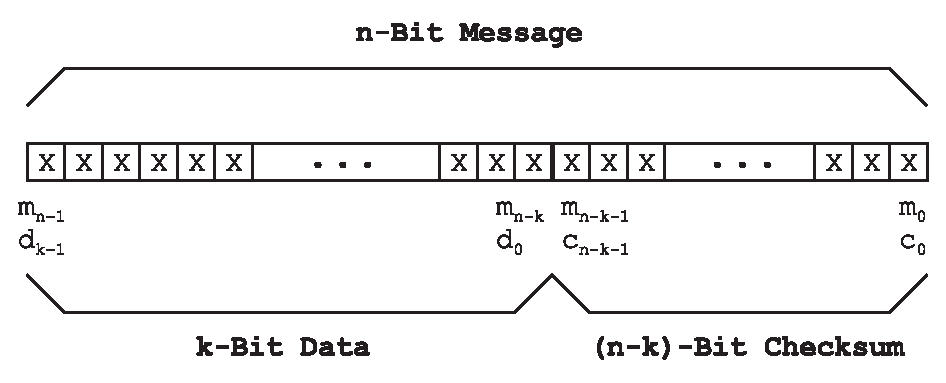
\includegraphics[width=4.6in]{c_edc0/cword02.eps}
\caption{Message Consisting Of The Concatenation Of $k$ Data Bits And $n-k$
         Check Bits, With Bit Notational Conventions For Cyclic Code Discusssion}
\label{fig:cedc0:scon0:sdpo0:01}
\end{figure}

A \index{cyclic code}\emph{cyclic code} is a linear code such that whenever
the vector $[m_0 \; m_1 \; m_2 \; \ldots{} \; m_{n-1}]$ is in the code, 
$[m_1 \; m_2 \; m_3 \; \ldots{} \; m_0]$ is also in the code.  When
this definition is applied recursively, it means that for any codeword, all
cyclic shifts of the codeword are also in the code (that is, in fact, why
a \emph{cyclic} code is called a \emph{cyclic} code).  For example, if 
10001 is a codeword; then 00011, 00110, 01100, and 11000 must also be
codewords (notice that these last four codewords are left cyclic shifts of the 
first codeword).  Note that since the code is linear, all sums of codewords 
must also be codewords.

A cyclic code is characterized by a generator polynomial, which we call
$g(x)$, of the form 

\begin{equation}
\label{eq:cedc0:scco0:sdpo0:01}
g(x) = g_{n-k} x_{n-k} + g_{n-k-1} x_{n-k-1} + \; \ldots \; + g_1 x + g_0,
\end{equation}

\noindent{}a polynomial of degree $n-k$, naturally containing up to $n-k+1$ terms.
Each coefficient $g_{n-k} \ldots g_{0}$ is chosen from $GF(2)$, so that
$g_{n-k} \ldots g_{0} \in \mathbb{B} = \{ 0 , 1 \}$.  We assume that
$g_{n-k}$ and $g_{0}$ are both 1.  We explain how the generator polynomial
specifies the code beginning in Section \ref{cedc0:scco0:ssut0}.

Cyclic codes are harnessed in two distinct ways, which we will call
the \emph{strong} and \emph{weak} ways.

In \emph{strong} utilization of cyclic codes
(Section \ref{cedc0:scco0:ssut0}), we must choose $g(x)$ in a very
special way with respect to $n$, and we cannot increase
$n$ arbitrarily (i.e. we are confined to messages of $n$ or
fewer bits).  If we choose $g(x)$ in this way, we can
control the minimum Hamming distance $\hat{d}$ of the cyclic code we specify.
We call this utilization \emph{strong} because we are able to preserve a 
strong property, the minimum Hamming distance $\hat{d}$ of the resulting code
(this is a very desirable feature, as it is in general not easy to construct a code
with a desirable large $\hat{d}$, and the theory of cyclic codes provides a way to do
this).
A typical ``strong'' utilization of a cyclic code may be in a communication peripheral
which can only accomodate a message of maximum length $\leq n$, and in this case
we can preserve strong properties of the cyclic code.

In \emph{weak} utilization of cyclic codes
(Section \ref{cedc0:scco0:swut0}), $n$ is unconstrained, and the minimum Hamming
distance of the code may degrade as far as $\hat{d}=2$ as $n$ is
increased.  We call such a utilization
\emph{weak} because only a \emph{weak} set of desirable properties can be preserved
in the resulting code.  A typical example of a weak utilization would be the CRC-32 (a
32-bit checksum) used to signature large files.  Such a utilization usually cannot
achieve even $\hat{d} = 3$, but can still preserve a low probability of undetected corruption
and protection against certain types of burst errors.

Note that the choice of generator polynomial $g(x)$ 
affects the properties of the code in both
the strong and weak utilizations, but in different ways.


%%%%%%%%%%%%%%%%%%%%%%%%%%%%%%%%%%%%%%%%%%%%%%%%%%%%%%%%%%%%%%%%%%%%%%%%%%%%%%%%
%%%%%%%%%%%%%%%%%%%%%%%%%%%%%%%%%%%%%%%%%%%%%%%%%%%%%%%%%%%%%%%%%%%%%%%%%%%%%%%%
%%%%%%%%%%%%%%%%%%%%%%%%%%%%%%%%%%%%%%%%%%%%%%%%%%%%%%%%%%%%%%%%%%%%%%%%%%%%%%%%
\subsection{\emph{Strong} Utilization Of Cyclic Codes}
%Subsection tag: sut0
\label{cedc0:scco0:ssut0}

In the strong utilization of a cyclic code,
the vector corresponding to the generator polynomial $g(x)$, 
$[0 \; \ldots \; 0 \; g_{n-k} \; g_{n-k-1} \; \ldots \; g_{0}]$ must 
be in the code, as must all of its cyclic shifts and sums of its
cyclic shifts.  A generator
matrix (not in standard form, and of course not the only generator 
matrix) for a cyclic code is of the form

\begin{equation}
\label{eq:cedc0:scco0:ssut0:02}
G = \left[
    \begin{array}{lllllllll}
    g_{n-k}  & g_{n-k-1}  & g_{n-k-2} &  \cdots  & g_{0}     &  0         &       0    &  \cdots{}  &   0 \\
    0        & g_{n-k}    & g_{n-k-1} &  \cdots  & g_{1}     &  g_{0}     &       0    &  \cdots{}  &   0 \\
    0        &   0        & g_{n-k}   &  \cdots  & g_{2}     &  g_{1}     &   g_{0}    &  \cdots{}  &   0 \\
    \vdots{} &            &           &          &           &            &            &            &     \\
    0        &   0        &   0       &  \cdots  &           &            &            &  \cdots{}  &   g_{0}   
    \end{array}
    \right]_{k \times n} \!\!\!\!\!\!\!\!\!\!.
\end{equation}

\noindent{}Note that the generator matrix in (\ref{eq:cedc0:scco0:ssut0:02})
has rows which are cyclic shifts of the coefficients of $g(x)$ (and 
for reasons discussed later, the other cyclic
shifts are also in the code).  Note also that $G$ is a
$k \times n$ matrix, consistent with (\ref{eq:cedc0:slco0:sgma0:01b}).

It is apparent from (\ref{eq:cedc0:scco0:ssut0:02}) that G can be
transformed into the form of (\ref{eq:cedc0:slco0:sgma0:01}) by
elementary row operations.  Two arguments can be
made.  First, by theorem, the determinant of an upper triangular matrix
(the first $k$ columns of $G$) is the product of the diagonal elements, 
and since we've assumed $g_0 = g_{n-k} = 1$, this determinant is necessarily 1.
Since the first $k$ columns of $G$ have full rank, they can be transformed
into $I_{k \times k}$.  Second, it is clear using elementary row operations how
to transform the first $k$ columns of $G$ into 
$I_{k \times k}$ (Exercise \ref{exe:cedc0:sexe0:03}).

\begin{vworkexamplestatement}
\label{ex:cedc0:scco0:ssut0:01}
For the $(7,4)$ code characterized by the generator polynomial 
$g(x) = 1 + x + x^3$, form the generator matrix of the code
as in (\ref{eq:cedc0:scco0:ssut0:02}), reduce it by elementary
row operations to the form of (\ref{eq:cedc0:slco0:sgma0:01}), 
and enumerate the $2^k = 16$ codewords.
\end{vworkexamplestatement}
\begin{vworkexampleparsection}{Solution}
With generator polynomial $g(x) = 1 + x + x^3$, $g_0 = 0$, $g_1 = 1$, 
$g_2 = 0$, and $g_3 = 1$.  By (\ref{eq:cedc0:scco0:ssut0:02}),

\begin{equation}
\label{eq:ex:cedc0:scco0:ssut0:01:01}
G = \left[
    \begin{array}{ccccccc}
    g_0 & g_1 & g_2 & g_3 &   0 &   0 &   0    \\
      0 & g_0 & g_1 & g_2 & g_3 &   0 &   0    \\
      0 &   0 & g_0 & g_1 & g_2 & g_3 &   0    \\
      0 &   0 &   0 & g_0 & g_1 & g_2 & g_3
    \end{array}
    \right] 
    =
    \left[
    \begin{array}{ccccccc}
      1 &   1 &   0 &   1 &   0 &   0 &   0    \\
      0 &   1 &   1 &   0 &   1 &   0 &   0    \\
      0 &   0 &   1 &   1 &   0 &   1 &   0    \\
      0 &   0 &   0 &   1 &   1 &   0 &   1
    \end{array}
    \right] .
\end{equation}

Adding (in the sense of $GF(2)$, see Section \ref{cedc0:sfft0:dff0})
the second row to the first yields

\begin{equation}
\label{eq:ex:cedc0:scco0:ssut0:01:02}
G = \left[
    \begin{array}{ccccccc}
      1 &   0 &   1 &   1 &   1 &   0 &   0    \\
      0 &   1 &   1 &   0 &   1 &   0 &   0    \\
      0 &   0 &   1 &   1 &   0 &   1 &   0    \\
      0 &   0 &   0 &   1 &   1 &   0 &   1
    \end{array}
    \right] .
\end{equation}

Adding the third row to the first row and to the second row (two
row operations) yields

\begin{equation}
\label{eq:ex:cedc0:scco0:ssut0:01:03}
G = \left[
    \begin{array}{ccccccc}
      1 &   0 &   0 &   0 &   1 &   1 &   0    \\
      0 &   1 &   0 &   1 &   1 &   1 &   0    \\
      0 &   0 &   1 &   1 &   0 &   1 &   0    \\
      0 &   0 &   0 &   1 &   1 &   0 &   1
    \end{array}
    \right] .
\end{equation}

Finally, adding the fourth row to the second row and to the third row (two
row operations) yields

\begin{equation}
\label{eq:ex:cedc0:scco0:ssut0:01:04}
G = \left[
    \begin{array}{ccccccc}
      1 &   0 &   0 &   0 &   1 &   1 &   0    \\
      0 &   1 &   0 &   0 &   0 &   1 &   1    \\
      0 &   0 &   1 &   0 &   1 &   1 &   1    \\
      0 &   0 &   0 &   1 &   1 &   0 &   1
    \end{array}
    \right] .
\end{equation}

The $2^4 = 16$ codewords can be enumerated by forming all linear combinations
of the rows of any of the matrices 
(\ref{eq:ex:cedc0:scco0:ssut0:01:01})
through (\ref{eq:ex:cedc0:scco0:ssut0:01:04}).  These 16 codewords are
enumerated in Table \ref{tbl:ex:cedc0:scco0:ssut0:01:01}.

\begin{table}
\caption{$2^4 = 16$ Codewords For Code Of Example \ref{ex:cedc0:scco0:ssut0:01}}
\label{tbl:ex:cedc0:scco0:ssut0:01:01}
\begin{center}
\begin{tabular}{|c|c|}
\hline
Data                      & Codeword  \\
(Value Of $k$ Data Bits)  &           \\
\hline
\hline
 0             &  0000 000 \\
\hline
 1             &  0001 101 \\
\hline
 2             &  0010 111 \\
\hline
 3             &  0011 010 \\
\hline
 4             &  0100 011 \\
\hline
 5             &  0101 110 \\
\hline
 6             &  0110 100 \\
\hline
 7             &  0111 001 \\
\hline
 8             &  1000 110 \\
\hline
 9             &  1001 011 \\
\hline
10             &  1010 001 \\
\hline
11             &  1011 100 \\
\hline
12             &  1100 101 \\
\hline
13             &  1101 000 \\
\hline
14             &  1110 010 \\
\hline
15             &  1111 111 \\
\hline
\end{tabular}
\end{center}
\end{table}
\end{vworkexampleparsection}
\vworkexamplefooter{}



%%%%%%%%%%%%%%%%%%%%%%%%%%%%%%%%%%%%%%%%%%%%%%%%%%%%%%%%%%%%%%%%%%%%%%%%%%%%%%%%
%%%%%%%%%%%%%%%%%%%%%%%%%%%%%%%%%%%%%%%%%%%%%%%%%%%%%%%%%%%%%%%%%%%%%%%%%%%%%%%%
%%%%%%%%%%%%%%%%%%%%%%%%%%%%%%%%%%%%%%%%%%%%%%%%%%%%%%%%%%%%%%%%%%%%%%%%%%%%%%%%
\subsection{\emph{Weak} Utilization Of Cyclic Codes}
%Subsection tag: wut0
\label{cedc0:scco0:swut0}


%%%%%%%%%%%%%%%%%%%%%%%%%%%%%%%%%%%%%%%%%%%%%%%%%%%%%%%%%%%%%%%%%%%%%%%%%%%%%%%%
%%%%%%%%%%%%%%%%%%%%%%%%%%%%%%%%%%%%%%%%%%%%%%%%%%%%%%%%%%%%%%%%%%%%%%%%%%%%%%%%
%%%%%%%%%%%%%%%%%%%%%%%%%%%%%%%%%%%%%%%%%%%%%%%%%%%%%%%%%%%%%%%%%%%%%%%%%%%%%%%%
\subsection{Perfect Codes}
%Subsection tag: pfc0
\label{cedc0:scob0:spfc0}

We define a \index{perfect code}\emph{perfect code} as a code 
where (\ref{eq:cedc0:scob0:rbc0:shsp0:01})
is an equality---that is, where the volume of the $2^k$ packing spheres precisely
consumes the $2^n$ messages available.  A perfect code has no ``waste'':  that is, 
there are no messages which do not participate in maintaining the required separation
between codewords.

In this section, we address two issues:

\begin{itemize}
\item The existence of integer solutions to

      \begin{equation}
      \label{eq:cedc0:scob0:spfc0:01}
      2^k V(n, \rho) = 2^n ,
      \end{equation}

      which is a question from number theory.

\item Given $n$,$k$ which satisfy (\ref{eq:cedc0:scob0:spfc0:01}), the existence
      of the codes whose possible existence is predicted.  It should be remembered
      that  (\ref{eq:cedc0:scob0:spfc0:01}) is a necessary but not sufficient 
      condition.
\end{itemize}


%%%%%%%%%%%%%%%%%%%%%%%%%%%%%%%%%%%%%%%%%%%%%%%%%%%%%%%%%%%%%%%%%%%%%%%%%%%%%%%%
%%%%%%%%%%%%%%%%%%%%%%%%%%%%%%%%%%%%%%%%%%%%%%%%%%%%%%%%%%%%%%%%%%%%%%%%%%%%%%%%
%%%%%%%%%%%%%%%%%%%%%%%%%%%%%%%%%%%%%%%%%%%%%%%%%%%%%%%%%%%%%%%%%%%%%%%%%%%%%%%%
\subsubsection[Existence Of Integer Solutions To 
               \protect\mbox{\protect$2^k V(n, \rho) = 2^n$}]
              {Existence Of Integer Solutions To 
               \protect\mbox{\protect\boldmath$2^k V(n, \rho) = 2^n$}}
%Subsubsection tag: pfc0
\label{cedc0:scob0:spfc0:seis0}



%%%%%%%%%%%%%%%%%%%%%%%%%%%%%%%%%%%%%%%%%%%%%%%%%%%%%%%%%%%%%%%%%%%%%%%%%%%%%%%%
%%%%%%%%%%%%%%%%%%%%%%%%%%%%%%%%%%%%%%%%%%%%%%%%%%%%%%%%%%%%%%%%%%%%%%%%%%%%%%%%
%%%%%%%%%%%%%%%%%%%%%%%%%%%%%%%%%%%%%%%%%%%%%%%%%%%%%%%%%%%%%%%%%%%%%%%%%%%%%%%%
\subsubsection{Existence Of Predicted Perfect Codes}
%Subsubsection tag: epc0
\label{cedc0:scob0:spfc0:sepc0}


%%%%%%%%%%%%%%%%%%%%%%%%%%%%%%%%%%%%%%%%%%%%%%%%%%%%%%%%%%%%%%%%%%%%%%%%%%%%%%%%
%%%%%%%%%%%%%%%%%%%%%%%%%%%%%%%%%%%%%%%%%%%%%%%%%%%%%%%%%%%%%%%%%%%%%%%%%%%%%%%%
%%%%%%%%%%%%%%%%%%%%%%%%%%%%%%%%%%%%%%%%%%%%%%%%%%%%%%%%%%%%%%%%%%%%%%%%%%%%%%%%
\section{Economical Implementation Of Linear Codes In Software}
%Section tag: eim0
\label{cedc0:seim0}


%%%%%%%%%%%%%%%%%%%%%%%%%%%%%%%%%%%%%%%%%%%%%%%%%%%%%%%%%%%%%%%%%%%%%%%%%%%%%%%%
%%%%%%%%%%%%%%%%%%%%%%%%%%%%%%%%%%%%%%%%%%%%%%%%%%%%%%%%%%%%%%%%%%%%%%%%%%%%%%%%
%%%%%%%%%%%%%%%%%%%%%%%%%%%%%%%%%%%%%%%%%%%%%%%%%%%%%%%%%%%%%%%%%%%%%%%%%%%%%%%%
\section[\protect\mbox{\protect$\hat{d}=2$} Codes Useful In Microcontroller Work]
        {\protect\mbox{\protect\boldmath$\hat{d}=2$} Codes Useful In Microcontroller Work}
%Section tag: dtc0
\label{cedc0:sdtc0}


%%%%%%%%%%%%%%%%%%%%%%%%%%%%%%%%%%%%%%%%%%%%%%%%%%%%%%%%%%%%%%%%%%%%%%%%%%%%%%%%
%%%%%%%%%%%%%%%%%%%%%%%%%%%%%%%%%%%%%%%%%%%%%%%%%%%%%%%%%%%%%%%%%%%%%%%%%%%%%%%%
%%%%%%%%%%%%%%%%%%%%%%%%%%%%%%%%%%%%%%%%%%%%%%%%%%%%%%%%%%%%%%%%%%%%%%%%%%%%%%%%
\section[\protect\mbox{\protect$\hat{d}=3$} Codes Useful In Microcontroller Work]
        {\protect\mbox{\protect\boldmath$\hat{d}=3$} Codes Useful In Microcontroller Work}
%Section tag: dhc0
\label{cedc0:sdhc0}



%%%%%%%%%%%%%%%%%%%%%%%%%%%%%%%%%%%%%%%%%%%%%%%%%%%%%%%%%%%%%%%%%%%%%%%%%%%%%%%%
%%%%%%%%%%%%%%%%%%%%%%%%%%%%%%%%%%%%%%%%%%%%%%%%%%%%%%%%%%%%%%%%%%%%%%%%%%%%%%%%
%%%%%%%%%%%%%%%%%%%%%%%%%%%%%%%%%%%%%%%%%%%%%%%%%%%%%%%%%%%%%%%%%%%%%%%%%%%%%%%%
\section{Acknowledgements}
\label{cedc0:sack0}

I'm very grateful to the following individuals who contributed insight
about error-detecting and error-correcting
codes on \index{comp.arch.embedded@\texttt{comp.arch.embedded}}\texttt{comp.arch.embedded}
and other
newsgroups:
Alan Coppola,
Eric Doenges,
Glen Herrmannsfeldt,
Dan Kotlow,
John Larkin,
Steven Murray,
Sphero Pefhany,
Jan-Hinnerk Reichert,
Thad Smith,
and
Jim Stewart.

I'm grateful to 
\index{Sperber, Ron}   Ron Sperber   \cite{bibref:i:ronsperber} and
\index{Chapman, Robin} Robin Chapman \cite{bibref:i:robinchapman}
for assistance with field theory offered on the 
\texttt{sci.math} newsgroup \cite{bibref:n:scimathnewsgroup}.

I'm also grateful to Mr. Michael J. Downes of the 
\index{comp.text.tex@\texttt{comp.text.tex}}\texttt{comp.text.tex} 
newsgroup, who assisted me with a technical difficulty involving
the \LaTeX ``$\backslash$\texttt{protect}'' command.


%%%%%%%%%%%%%%%%%%%%%%%%%%%%%%%%%%%%%%%%%%%%%%%%%%%%%%%%%%%%%%%%%%%%%%%%%%%%%%%%
%%%%%%%%%%%%%%%%%%%%%%%%%%%%%%%%%%%%%%%%%%%%%%%%%%%%%%%%%%%%%%%%%%%%%%%%%%%%%%%%
%%%%%%%%%%%%%%%%%%%%%%%%%%%%%%%%%%%%%%%%%%%%%%%%%%%%%%%%%%%%%%%%%%%%%%%%%%%%%%%%
\section{Exercises}
\label{cedc0:sexe0}

\begin{vworkexercisestatement}
\label{exe:cedc0:sexe0:01}
Show that the minimum Hamming distance of the code $\{0001, 0110, 1010, 1101\}$
is 2.
\end{vworkexercisestatement}

\begin{vworkexercisestatement}
\label{exe:cedc0:sexe0:02}
Verify Equation \ref{eq:cedc0:shco0:02}.
\end{vworkexercisestatement}

\begin{vworkexercisestatement}
\label{exe:cedc0:sexe0:03}
Outline a procedure for transforming the $G$ of 
(TBD%
%\ref{eq:cedc0:scco0:sdpo0:02}%
) into 
the form of (\ref{eq:cedc0:slco0:sgma0:01}).
\end{vworkexercisestatement}
\vworkexercisefooter{}

\vworkexercisefooter{}

%End of file c_edc0.tex

